\chapter[QTL mapping in outbred rat population with imbalanced founder allele frequencies]{QTL mapping in outbred rat population with imbalanced \\ founder allele frequencies
\footnote{This chapter has been adapted from a paper published in Obesity. The citation will be as follows: Keele, G. R., Prokop, J. W., He, H., Holl, K., Littrell, J., Deal, A., Francic, S., Cui, L., Gatti, D. M., Broman, K. W., Tschannen, M., Tsaih, S.-W., Zagloul, M., Kim, Y., Baur, B., Fox, J., Robinson, M., Levy, S., Flister, M. J., Mott, R., Valdar, W., and Solberg Woods, L. C. (2018). Genetic Fine-Mapping and Identification of Candidate Genes and Variants for Adiposity Traits in Outbred Rats. Obesity, 26(1):213-222.}}
\label{chap:hs_rats}

\section{Introduction}

Obesity and overweight are major risk factors for multiple cardiovascular and metabolic diseases \citep{Wang2009}. Of particular importance is visceral, or abdominal, adipose tissue, which is strongly predictive of metabolic health \citep{Emdin2017a}.  Multiple environmental (e.g., lifestyle) and genetic factors contribute to obesity with genetics accounting for up to 70\% of the population variance for human body mass index (BMI) and obesity \citep{Stunkard1986} and visceral adiposity \citep{Katzmarzyk2000}. To date, human genome-wide association studies have identified many genes for anthropomorphic traits \citep{Locke2015, Lu2016, Ng2017, Speliotes2010}, but these genes explain only a small proportion of the heritable variation \citep{Locke2015}, indicating many genes are yet unidentified. Identification of additional genes is particularly important because there has been a steady increase in prevalence of overweight and obesity since the 1970's \citep{Wang2009}, with over one third of adults and almost one fifth of all children in the United States being classified as obese \citep{Flegal2016}.   

One strategy for identifying the heritable modifiers of obesity is to control for exogenous environmental factors using experimental genetic mapping strategies such as the outbred heterogeneous stock (HS) rats. HS rats descend from eight inbred founder strains and have been out-bred for over 70 generations, such that the fine recombination block structure allows genetic mapping to identify regions that are only a few Mb \citep{SolbergWoods2014}. In previous work, we used HS rats to fine-map a single region on rat chromosome 1 previously identified for glucose and insulin traits \citep{SolbergWoods2010, SolbergWoods2012}, and identified \textit{Tpcn2} as a likely causal gene at this locus \citep{Tsaih2014}. Here, we demonstrate that HS rats vary for adiposity traits including body weight and visceral fat pad weight, and that these measures correlate with metabolic health. We then detect and fine-map QTL for these traits genome-wide and identify five likely causal genes within these loci.

\section{Methods and Procedures}

\subsection{Animals}

\subsubsection{Heterogeneous stock colony}

The NMcwi:HS colony, hereafter referred to as HS, was initiated by the NIH in 1984 using the following eight inbred founder strains: ACI/N, BN/SsN, BUF/N, F344/N, M520/N, MR/N, WKY/N  and WN/N  \citep{Hansen1984}. This colony has been maintained at the Medical College of Wisconsin since 2006 and has been through over 70 generations of breeding. Rats were given ad libitum access to Teklad 5010 diet (Harlan Laboratories). Additional housing conditions are detailed in Detailed Methods.

\subsubsection{Founding inbred sub-strains}

Other than M520/N (now maintained at MCW), phenotyping of the founders was conducted in the following sub-strains (abbreviated names to be used throughout manuscript in parentheses): ACI/Eur or ACI/Seg (ACI), BN/SsnHsd (BN), BUF/NHsd (BUF), F344/NHsd (F344), and WKY/NHsd (WKY). We tested 8-19 male rats per inbred strain.

\subsection{Phenotyping protocol}

We measured body weight at 16 weeks of age in 989 male HS rats. Rats underwent an intra-peritoneal glucose tolerance test (IPGTT) as described previously \citep{SolbergWoods2010, SolbergWoods2012}. We used the Ascensia Elite system for reading blood glucose values (Bayer, Elkhart, IN). Plasma insulin levels were determined using an ultrasensitive ELISA kit (Alpco Diagnostics, Salem, NH). The following metabolic measures were calculated: area under the curve for glucose (glucose\_AUC) and insulin (insulin\_AUC) during the IPGTT, the quantitative insulin sensitivity check (QUICKI) as a measure of insulin sensitivity, and the insulinogenic index (IGI) as a measure of beta cell sensitivity to glucose \citep{SolbergWoods2012}. 

Inbreds and 743 HS rats were euthanized after an overnight fast at 17 weeks of age. Body weight and two measures of body length (from nose to base of the tail and from nose to end of tail) were collected, allowing us to calculate two measures of body mass index: BMI\_Tail\_Base and BMI\_Tail\_End. BMI was calculated as: (body weight/body length2)$\times$10. Rats were euthanized by decapitation and trunk blood was collected. Fasting cholesterol and triglycerides were determined from fasting serum on an ACE Alera autoanalyzer using an enzymatic method for detection. Several tissues were dissected and weighed including retroperitoneal and epididymal visceral fat pads, hereafter referred to as RetroFat and EpiFat, respectively. Liver and adipose tissues were snap-frozen in liquid nitrogen for subsequent expression analysis. All protocols were approved by the IACUC committee at MCW. Phenotyping data have been deposited in RGD (\url{www.rgd.mcw.edu}).

\subsection{Genotyping}

We extracted DNA from tail tissue from HS and the original eight inbred founder strains (tissue obtained from the NIH) using either the Qiagen DNeasy kit (Valencia, CA) or a phenol-chloroform extraction. Founder and HS rats were genotyped using the Affymetrix GeneChip Targeted Genotyping technology on a custom 10K SNP array panel as previously described \citep{STARConsortium2008}, with marker locations based on rat genome assembly 6.0. 147 samples were genotyped by the Vanderbilt Microarray Shared Resource center at Vanderbilt University in Tennessee (currently VANTAGE: \url{http://www.vmsr.edu}) and the remaining 842 by HudsonAlpha Institute (\url{http://hudsonalpha.org}). From the 10,846 SNPs on the array, 8,218 were informative and produced reliable genotypes in the HS rats. From these final informative markers, the average SNP spacing was 284 Kb, with an average heterozygosity of 25.68\%. Principle Component Analysis was used to confirm there were no systematic genotyping differences between the two centers (\textbf{Figure \ref{fig:pca}}).

\subsection{RNA-Seq}

RNA was extracted from liver of 398 HS rats using Trizol. Illumina kits were used to create library preps and RNA-Seq was run on the Illumina HiSeq 2500. RSEM and Bowtie were used to align reads and compute transcript level expression abundance (Detailed Methods).  

\section{Statistical Analysis}

\subsection{Estimating heritability of adiposity traits}

Narrow-sense heritability was estimated for each transformed phenotype using a Bayesian linear mixed model (LMM) implemented in INLA \citep{Holand2013a, Rue2009a}. The LMM included fixed effects representing time food deprived, order of tissue harvest, and dissector (notably, dissector significantly affected EpiFat and BMI\_Tail\_Base), and a random ``polygenic" effect, which represented the effect of overall relatedness (calculated as in \cite{Gatti2014}). Heritability, $h^2$, was defined as the proportion of variance attributed to polygenic effects vs residual noise (Detailed Methods).

\subsection{Genome-wide association}

QTL were identified by genome-wide association of imputed allele dosages of genotyped SNPs. A hidden Markov model \citep{Broman2016} was used to infer each HS rat's haplotype mosaic and thereby obtain robust estimates of the genotype of each SNP. Association tests were then performed, SNP-by-SNP, on each trait using a frequentist version of the LMM described for estimating heritability but with an added SNP effect term. Tests of the SNP effect yielded p-values that are here reported as negative log to the base 10, or ``logP". Genome-wide significance thresholds for logP scores were estimated by parametric bootstrap samples from the fitted null \citep{SolbergWoods2010, Valdar2009}.  Linkage Disequilibrium (LD) intervals for the detected QTL were defined by including neighboring markers that met a set level of LD, measured with the squared correlation coefficient $r^{2}$; we used $r^{2}=0.5$ to define intervals based on the plots of the SNP associations overlaid with LD information (Detailed Methods).

\subsection{Fine-mapping and haplotype effect estimation at detected QTL}

SNP variants within the LD interval were prioritized used the multi-SNP method LLARRMA-dawg \citep{Sabourin2015}, which calculates for each SNP a resample model inclusion probability (RMIP):  SNPs with high RMIPs represent strong, independent signals, and the existence of multiple SNPs with a high RMIP is consistent with the presence of multiple independent signals. To characterize each QTL signal, we used the Diploffect model \citep{Zhang2014}, which estimates the relative contributions of alternate founder haplotypes (Detailed Methods).

\subsection{Candidate gene identification}

Two parallel approaches were used: 1) bioinformatic analysis and protein modeling of known sequence variants; and, 2) mediation analysis of expression levels. For (1), we used HS founder sequence (\url{www.rgd.mcw.edu}; genome build Rn6) to identify highly conserved, non-synonymous coding variants within each QTL that were predicted to be damaging by Polyphen (\url{http://genetics.bwh.harvard.edu/pph/}) and/or SIFT, focusing on variants in founder strains that showed haplotype effects at the locus. Variants were confirmed using Sanger sequencing and then analyzed in the Sequence-to-Structure-to-Function analysis as previously described \citep{Prokop2017}.  Briefly, proteins were assessed with codon selection analysis of multiple species open reading frames, inspected for linear motif impact near variants of interest, and modeled with I-TASSER \citep{Roy2010} and YASARA \citep{Krieger2009}. Models were then assessed for likely impact on protein folding and/or function based on model confidence, phylogenetic sequence alignment, conservation, and whether or not the variant altered structural packing, molecular dynamic simulations, binding partners, linear motifs or post-translational modifications. For (2), transcript abundance levels of genes within HS liver were evaluated as potential causal mediators of the physiological QTL through mediation analysis \citep{Baron1986} (Detailed Methods).

\section{Results}

\subsection{HS founder strains exhibit large variation in adiposity traits}

All phenotypes were rank-inverse normal transformed except EpiFat, which instead was log transformed based on the Box-Cox procedure.  All traits differed significantly between the inbred founder strains: body weight ($F_{5, 76} = 15.492$, $p = \num{1.74e-10}$), BMI\_Tail\_End ($F_{5, 73} = 25.024$, $p = \num{1.34e-14}$), BMI\_Tail\_Base ($F_{5, 73} = 9.683$, $p = \num{4.02e-7}$), EpiFat ($F_{5, 78} = 69.541$, $p < \num{2.2e-16}$) and RetroFat ($F_{5, 78} = 38.157$, $p < \num{2.2e-16}$; \textbf{Figure \ref{fig:founder_data}}).  The BUF inbred strain had significantly more EpiFat mass (Tukey-Kramer $p < 0.05$) and BMI\_Tail\_End (Tukey-Kramer $p < 0.05$) relative to all other strains.  BUF also had significantly more RetroFat mass compared to all strains (Tukey-Kramer $p < 0.001$) except F344 (Tukey-Kramer $p = 0.06175$), higher body weight relative to ACI, BN, and M520 (Tukey-Kramer $p < 0.01$), and higher BMI\_Tail\_Base than ACI and M520 (Tukey-Kramer $p < 0.05$).  ACI, BN and M520 were the lightest strains, with BN and M520 showing significantly lighter EpiFat (Tukey-Kramer $p < \num{1e-5}$) and RetroFat (Tukey-Kramer $p < 0.001$) relative to other strains.

\begin{figure}
\centering
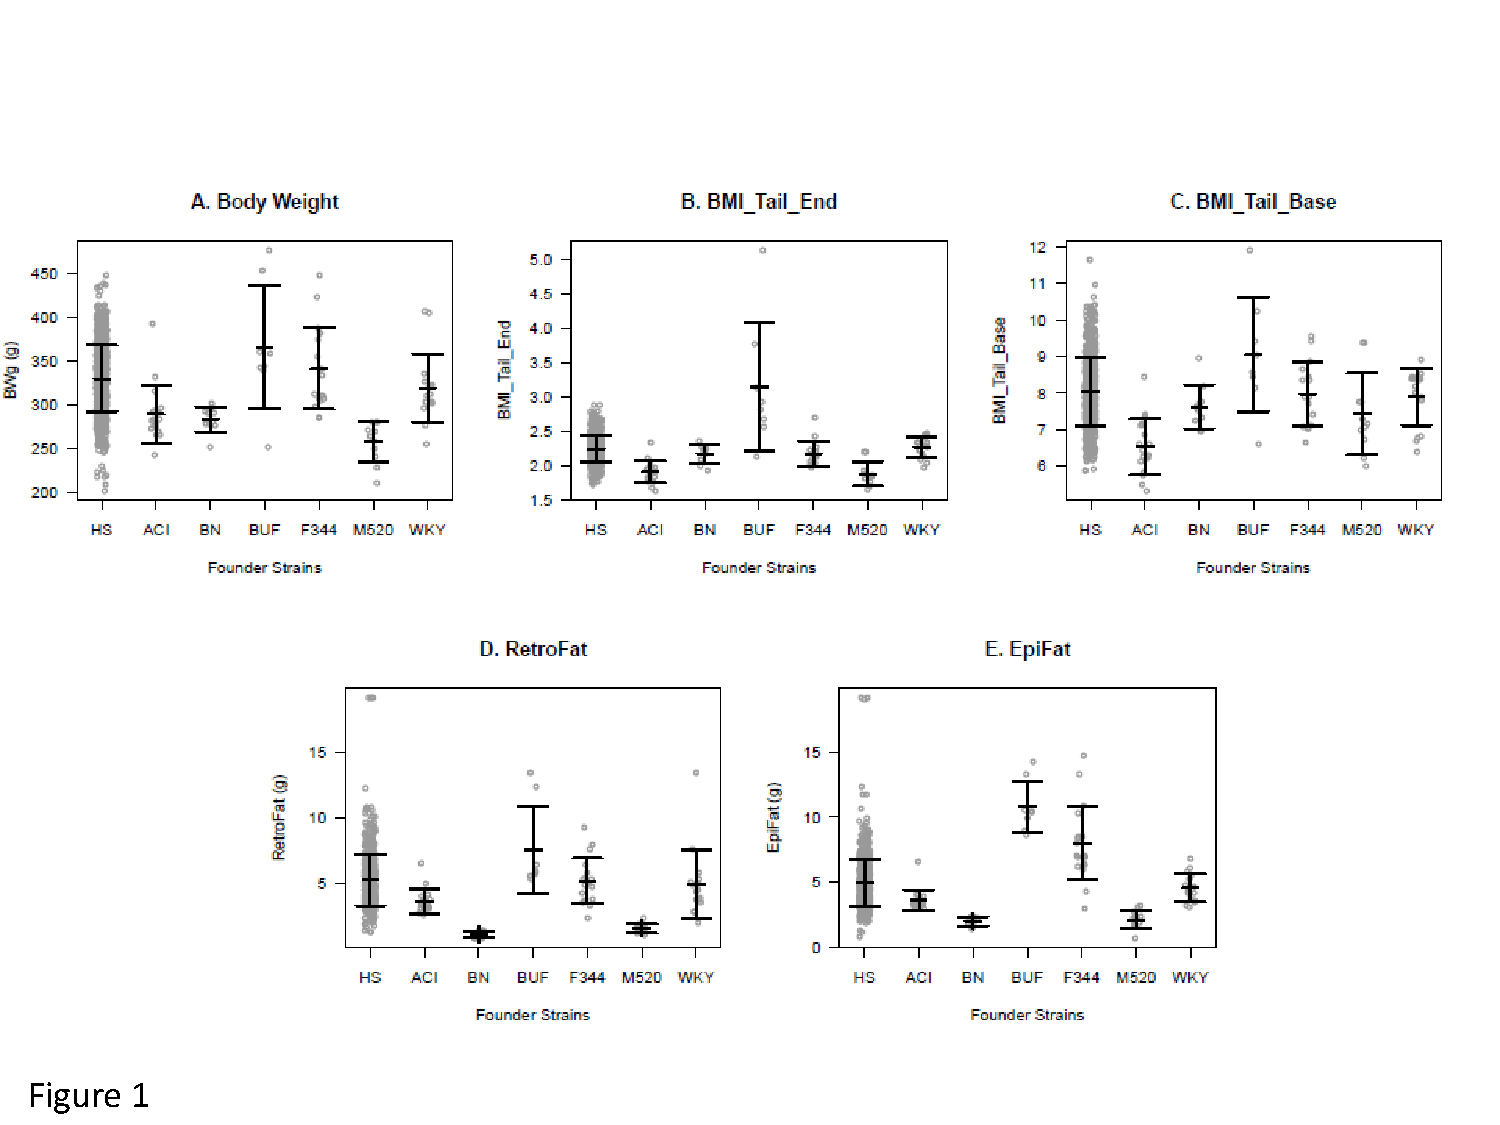
\includegraphics[trim={0in 0.8in 0in 1in}, clip, width=\textwidth]{figures/5-hsrats/Figure1.pdf}
\caption[Adiposity traits in the HS rats and the inbred founders]{Adiposity traits in inbred founders and HS rats. Mean + SD are shown. BMI is body mass index from nose to end of tail (BMI\_Tail\_End) and from nose to base of the tail (BMI\_Tail\_Base). EpiFat and RetroFat are epididymal and retroperitoneal fat pad weight, respectively. Gray circles represent individual animals from 8-19 individuals from 6 of the founder strains, and the HS rats (989 in body weight; 741 in RetroFat, EpiFat, and BMI\_Tail\_End; and 740 in BMI\_Tail\_Base). See text for statistical differences between founder strains. \label{fig:founder_data}}
\end{figure}

\subsection{Adiposity traits are highly correlated with measures of metabolic health in HS rats}

Variation between the founder strains is represented within the HS colony (\textbf{Figure \ref{fig:founder_data}}). Adiposity measures were highly correlated with several measures of metabolic health (\textbf{Table \ref{tab:cor}}, \textbf{Figure \ref{fig:adiposity_cor}}). EpiFat significantly correlated with every measure of metabolic health and RetroFat correlated with all but fasting glucose. Body weight significantly correlated with all measures except fasting triglycerides. BMI\_Tail\_End significantly correlated with fasting total cholesterol, fasting tricglycerides, glucose AUC, insulin AUC, and IGI, whereas BMI\_Tail\_Base did not significantly correlate with any of the measures of metabolic health.

\begin{table}
\centering
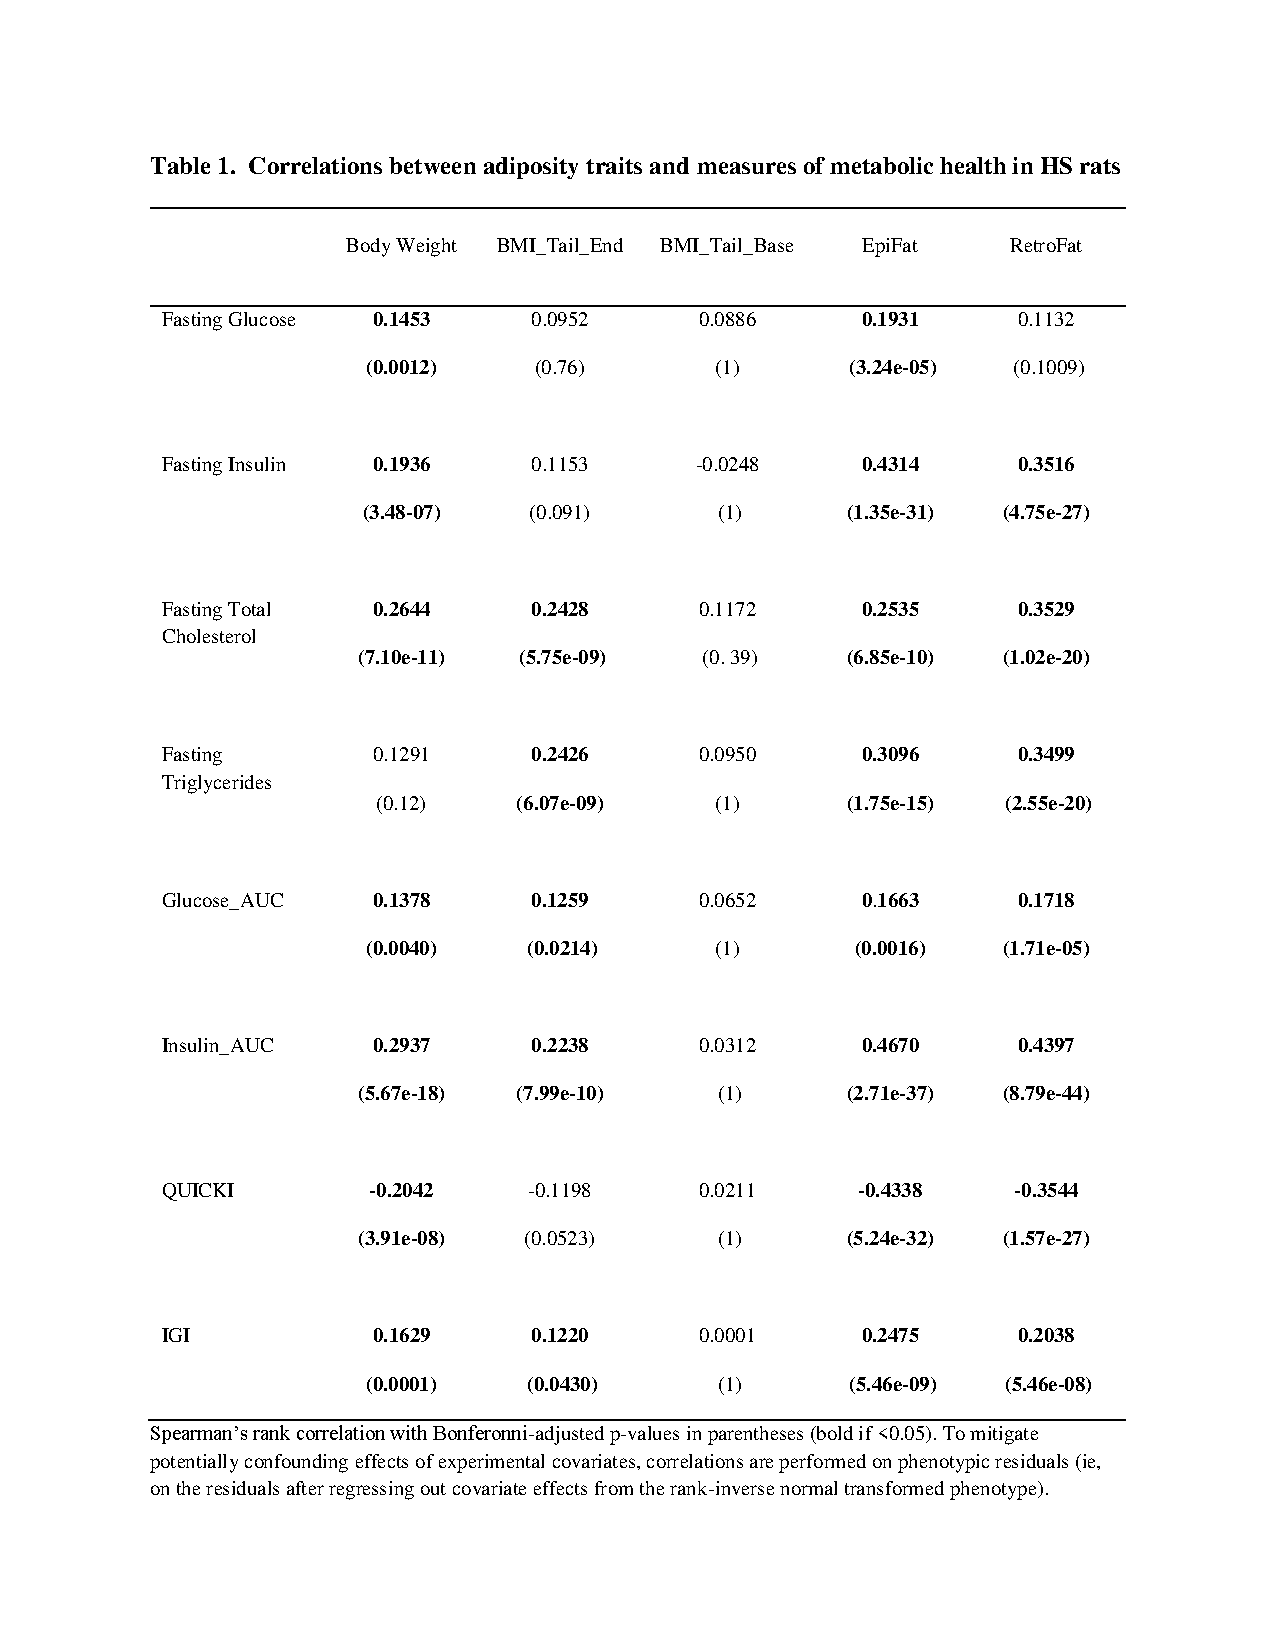
\includegraphics[trim={0in 1in 0in 1.2in}, clip, width=\textwidth]{figures/5-hsrats/Table1.pdf}
\caption{Correlations between adiposity and measures of metabolic health in HS rats \label{tab:cor}}
\end{table}

\begin{figure}
\centering
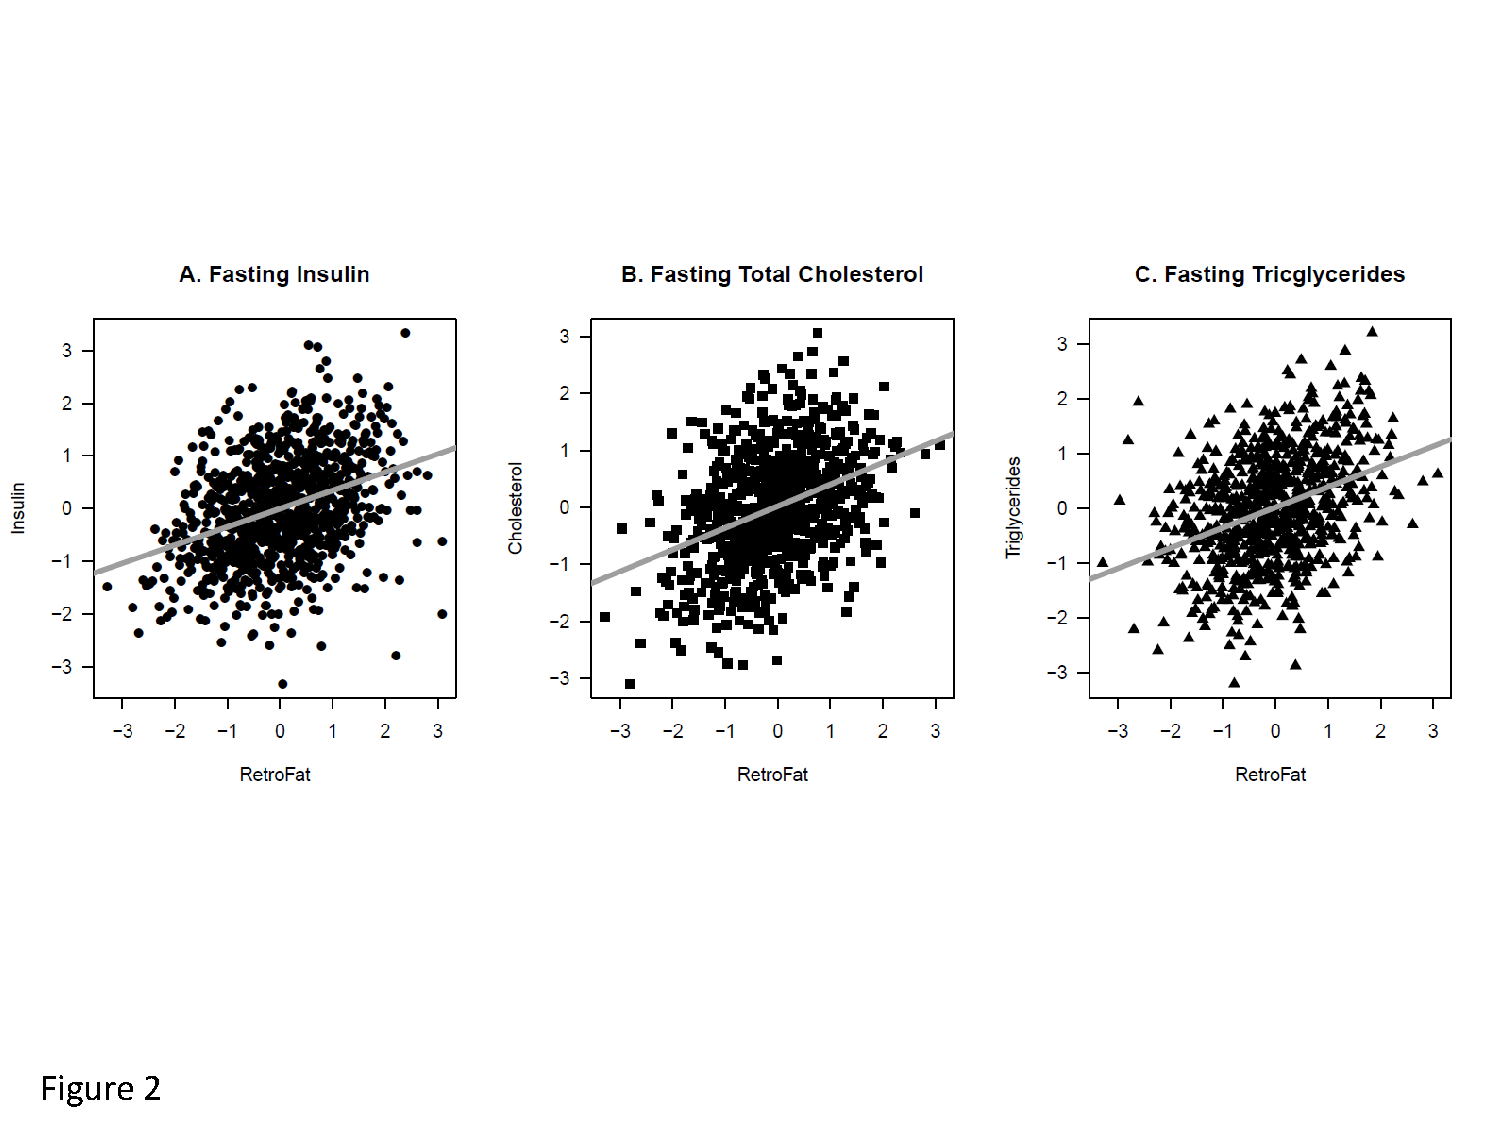
\includegraphics[trim={0in 2in 0in 1.5in}, clip, width=\textwidth]{figures/5-hsrats/Figure2.pdf}
\caption[Significant correlations between adiposity and metabolic traits in HS rats]{Significant correlations between RetroFat (retroperitoneal fat pad weight) and A) fasting insulin ($p = \num{4.75e-27}$), B) fasting total cholesterol ($p = \num{1.02e-20}$) and C) fasting triglycerides ($p = \num{2.55e-20}$) in HS rats. Plots show the residuals of rank-inverse normal transformed phenotypes with nuisance factors regressed out to restrict correlation estimates to that between RetroFat and these metabolic traits. Significant correlations were also found between RetroFat and several other measures of metabolic health (see \textbf{Table \ref{tab:cor}}). \label{fig:adiposity_cor}}
\end{figure}

\subsection{Adiposity traits are highly heritable}

Adiposity traits were highly heritable in HS rats: body weight (posterior mode of $h^{2} = 75.3\%$; 95\% highest posterior density interval$ = 67.0-81.7\%$), EpiFat ($54.1\%$; $40.1-66.0\%$), RetroFat ($53.9\%$; $39.7-66.7\%$), BMI\_Tail\_End ($45.0\%$; $32.3-57\%$) and BMI\_Tail\_Base ($25.4\%$; $13.6-41.8\%$).

\subsection{RetroFat QTL on chromsomes 1 and 6}

Two 90\% significant QTL were identified for RetroFat, a QTL on rat chromosome 6: 22.79-28.93 Mb (6.14 Mb, $\text{logP} = 4.73$) and a QTL on chromosome 1: 280.63 - 281.82 Mb (1.19 Mb, $\text{logP} = 4.69$; \textbf{Figures \ref{fig:retrofat_chr6}ABC}, \textbf{\ref{fig:retrofat_chr1}ABC}).  The LLARRMA-dawg multi-SNP fine-mapping analysis narrowed the most likely region of the broader chromosome 6 QTL to 1.46 Mb region (27.17 - 28.63 Mb; \textbf{Figure \ref{fig:llarrma}}) narrowing the number of the genes from 130 to 30 (\textbf{Tables \ref{tab:retrofat_chr6_genes_1}}-\textbf{\ref{tab:retrofat_chr6_genes_4}}, \textbf{Figure \ref{fig:annotations}}). Estimating founder haplotype effects at the chromosome 6 QTL gave an effect size (posterior median) of 11.05\% and showed that at this locus, decreased fat pad weight is associated with the WKY haplotype (\textbf{Figure \ref{fig:retrofat_chr6}D}).  For the chromosome 1 QTL the effect size was 13.33\%, with increased fat pad weight associated with BUF, MR and WKY haplotypes (\textbf{Figure \ref{fig:retrofat_chr1}D}). 

\subsection{Identification of \textit{Adcy3}, \textit{Krtcap3}, \textit{Slc30a3} within the chromosome 6 RetroFat QTL}

Within the chromosome 6 RetroFat QTL, bioinformatic analysis revealed only one gene, \textit{Adcy3}, that had a highly conserved, potentially damaging, non-synonymous variant in the WKY rat, the founder haplotype associated with decreased Retrofat at this locus. \textit{Adcy3} also falls within the fine-mapped support interval of the QTL (\textbf{Figure \ref{fig:retrofat_chr6}C}).  The WKY founder strain harbors a C at position 28,572,363 bp within \textit{Adcy3} while all other strains harbor a T, resulting in a leucine-to-proline substitution at amino acid 121.  Based on DNA information from 86 nucleotide sequences for ADCY3, this variant is highly conserved with evidence for selective pressure. Protein modeling indicated that amino acid 121 is located within the first transmembrane region, with a proline likely causing a bend in the helix and thus altered transmembrane packing (\textbf{Figure \ref{fig:retrofat_chr6}E}).

Because fine-mapping supported multiple independent signals at the QTL, we investigated potential mediators among the cis-expressed genes. Mediation analysis identified six potential mediators, all driven by the WKY haplotype (\textbf{Figure \ref{fig:mediation_analysis}}; \textbf{Tables \ref{tab:retrofat_chr6_potential_mediators}} and \textbf{\ref{tab:retrofat_chr6_candidate_mediators}}), suggesting that multiple genes may influence RetroFat at this locus. Two in particular were strongly supported:  \textit{Krtcap3} as a full mediator and \textit{Slc30a3} as a partial mediator, remaining significant after controlling for \textit{Krtcap3}. Under the proposed model (\textbf{Figure \ref{fig:mediation_graph}}), the WKY haplotype increases expression of \textit{Krtcap3}, which is itself negatively correlated with RetroFat (\textbf{Figure \ref{fig:krtcap3}}), and thus the causal path is consistent with the negative WKY effect on RetroFat at the locus; meanwhile, WKY decreases expression of \textit{Slc30a3}, which is also negatively correlated RetroFat, suggesting \textit{Slc30a3} is a suppressor of the QTL/\textit{Krtcap3} effect.

\begin{figure}
\centering
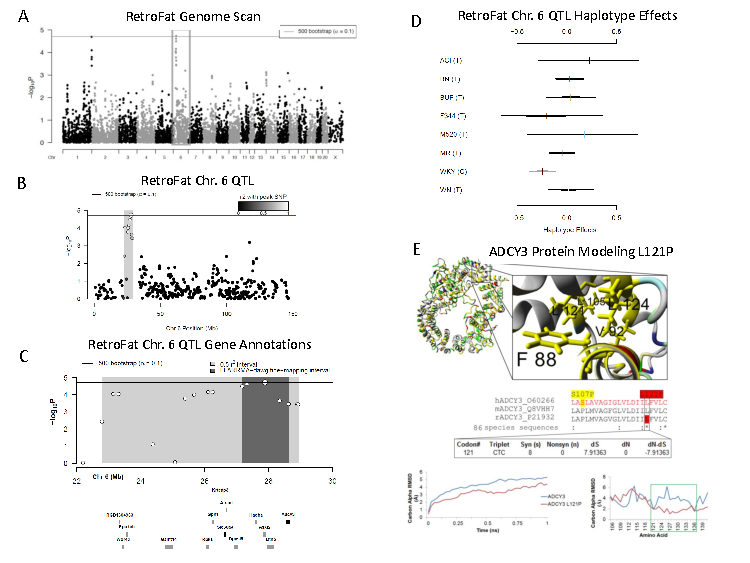
\includegraphics[trim={0in 0in 0in 0in}, clip, width=\textwidth]{figures/5-hsrats/Figure3-alt.pdf}
\caption[RetroFat chromosome 6 QTL and subsequent fine-mapping analyses]{Genome scan of RetroFat (A). X-axis is position on chromosome and y-axis is the logP level of association.  Genome-wide significance thresholds were calculated using parametric bootstraps from the null model ($\alpha=0.1$, $\text{logP} = 4.70$). The grey region highlights the 6.14 LD support interval of the chromosome 6 QTL showing neighboring markers that are correlated with the peak marker, representing genomic regions likely to contain the causal variant underlying the statistical signal (B). Annotation of genes that fall within the support interval (C). The entire 6.14 region is shaded in grey, with the fine-mapped 1.46 Mb region shaded in dark grey. Only genes that have a cis eQTL are shown.  All 130 genes within the region are listed in \textbf{Tables \ref{tab:retrofat_chr6_genes_1}}-\textbf{\ref{tab:retrofat_chr6_genes_4}}. Additive haplotype effects were estimated using the Diploffect model, which takes into account uncertainty in haplotype state (D). SNP allele information is overlaid on the haplotype effects, and are distinguished by black or gray. The WKY haplotype, the only haplotype with the C allele at the chromosome 6 locus, has a significantly negative effect on phenotype. Protein modeling for ADCY3 (E). Variant L121P of ADCY3 is found with the conserved hydrophobic core of the transmembrane helices.  A zoomed in view is shown to the right.  The middle panel shows sequence alignments of amino acids. ADCY3 amino acid 121 is also 100\% conserved (red) as a leucine in 86 analyzed vertebrate species. A human SNP is known at amino acid 107 (yellow). Using the DNA information from the 86 nucleotide sequences for ADCY3, there is also evidence of selective pressure in the DNA sequence to conserve the amino acid. Bottom panel shows molecular dynamic simulations for ADCY3. Simulations performed on the protein dimer for wild type (WT blue) or the mutant (ADCY3 L121P, red) suggests that the models' average movement over time is altered. Altered movement is seen in the simulations for ADCY3 with fluctuation of amino acids found near amino acid 121 when mutated. \label{fig:retrofat_chr6}}
\end{figure}

\begin{figure}
\centering
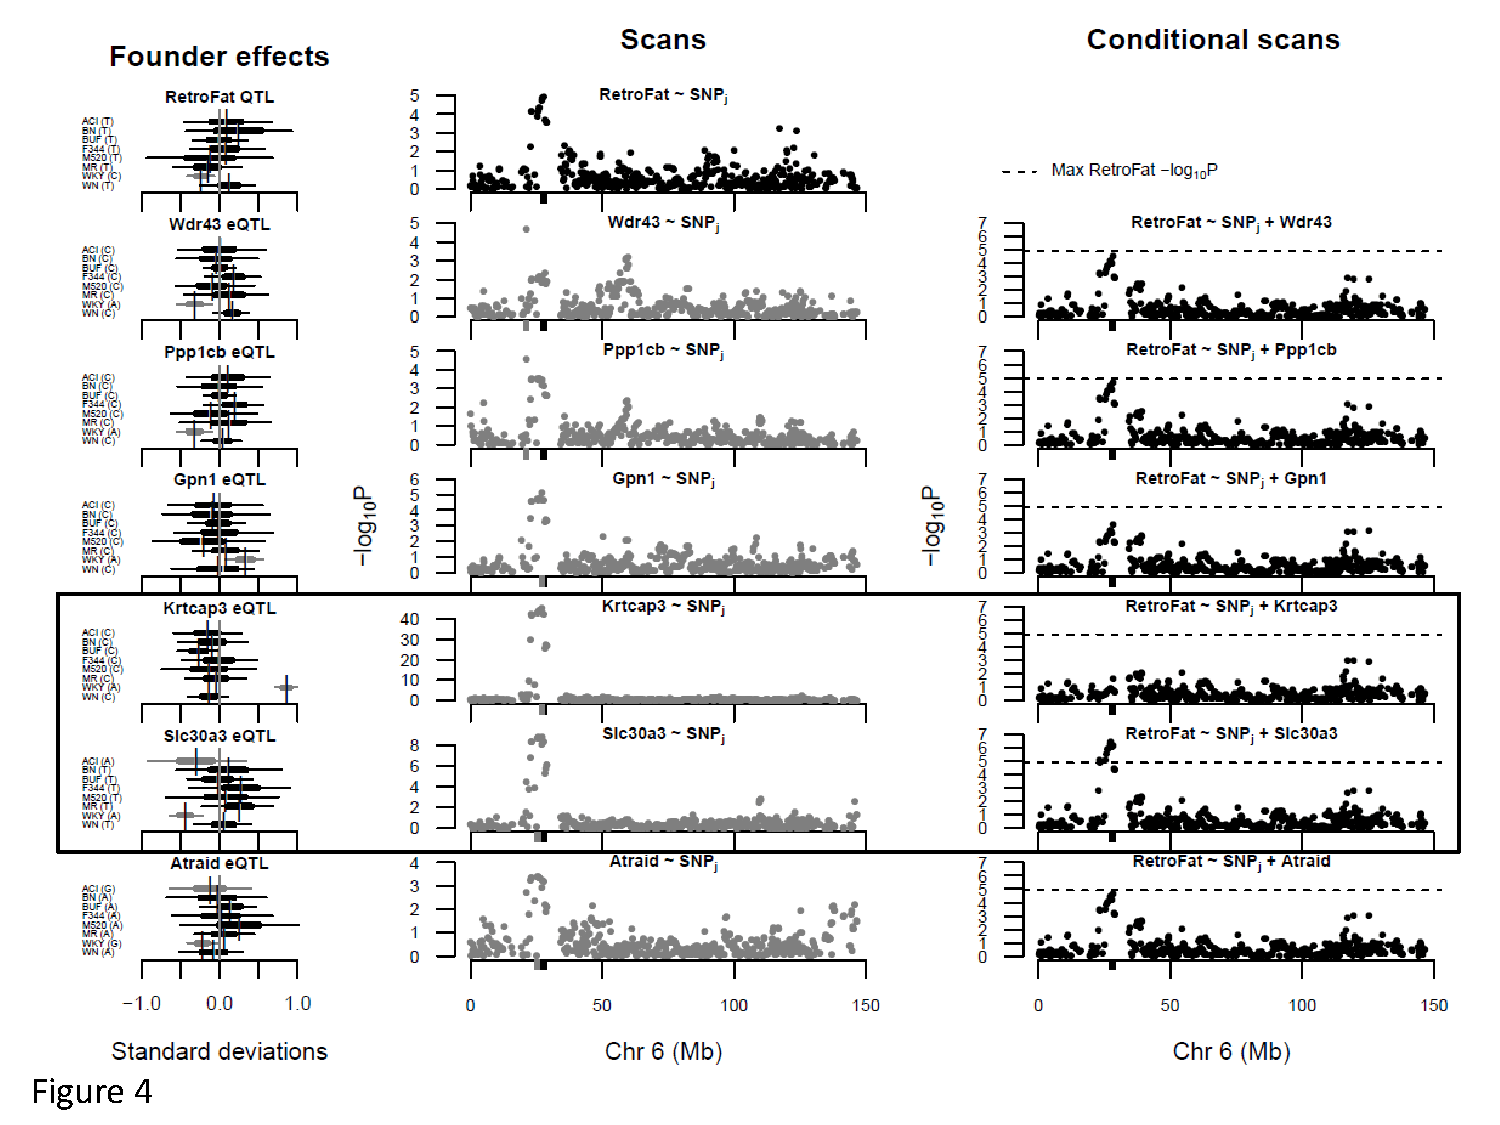
\includegraphics[trim={0in 0.3in 0in 0in}, clip, width=\textwidth]{figures/5-hsrats/Figure4.pdf}
\caption[Co-localizing eQTL and their effect on the QTL association with RetroFat when included in the model]{Mediation analysis identified the expression levels of six genes (\textit{Wdr43}, \textit{Ppp1cb}, \textit{Gpn1}, \textit{Krtcap3}, \textit{Slc30a3}, and \textit{Atraid}; \textbf{Table \ref{tab:retrofat_chr6_candidate_mediators}}) in the RetroFat chromosome 6 QTL interval as potential mediators of the QTL effect on the phenotype. [Middle column] Comparisons of the RetroFat chromosome 6 association scan with association scans for the potential mediators reveals them to likely have co-localizing cis eQTL with the RetroFat QTL. [Left column] The haplotype effects on RetroFat at the QTL and on the mediators at the eQTL reveals that in this region, the WKY haplotype is largely driving the differences in RetroFat and mediator gene expression, suggesting a possible connection between RetroFat and local gene expression. [Right column] RetroFat chromosome 6 association scans, conditioned on candidate gene expression, is consistent with the mediation analysis finding that \textit{Krtcap3} is a strong candidate as full mediator of the effect of QTL on RetroFat. When \textit{Krtcap3} expression is included in the model, the QTL is largely removed. \textit{Slc30a3}, as a potential suppressor of the QTL effect on RetroFat, actually increases the significance seen at the QTL. \label{fig:mediation_analysis}}
\end{figure}

\begin{figure}
\centering
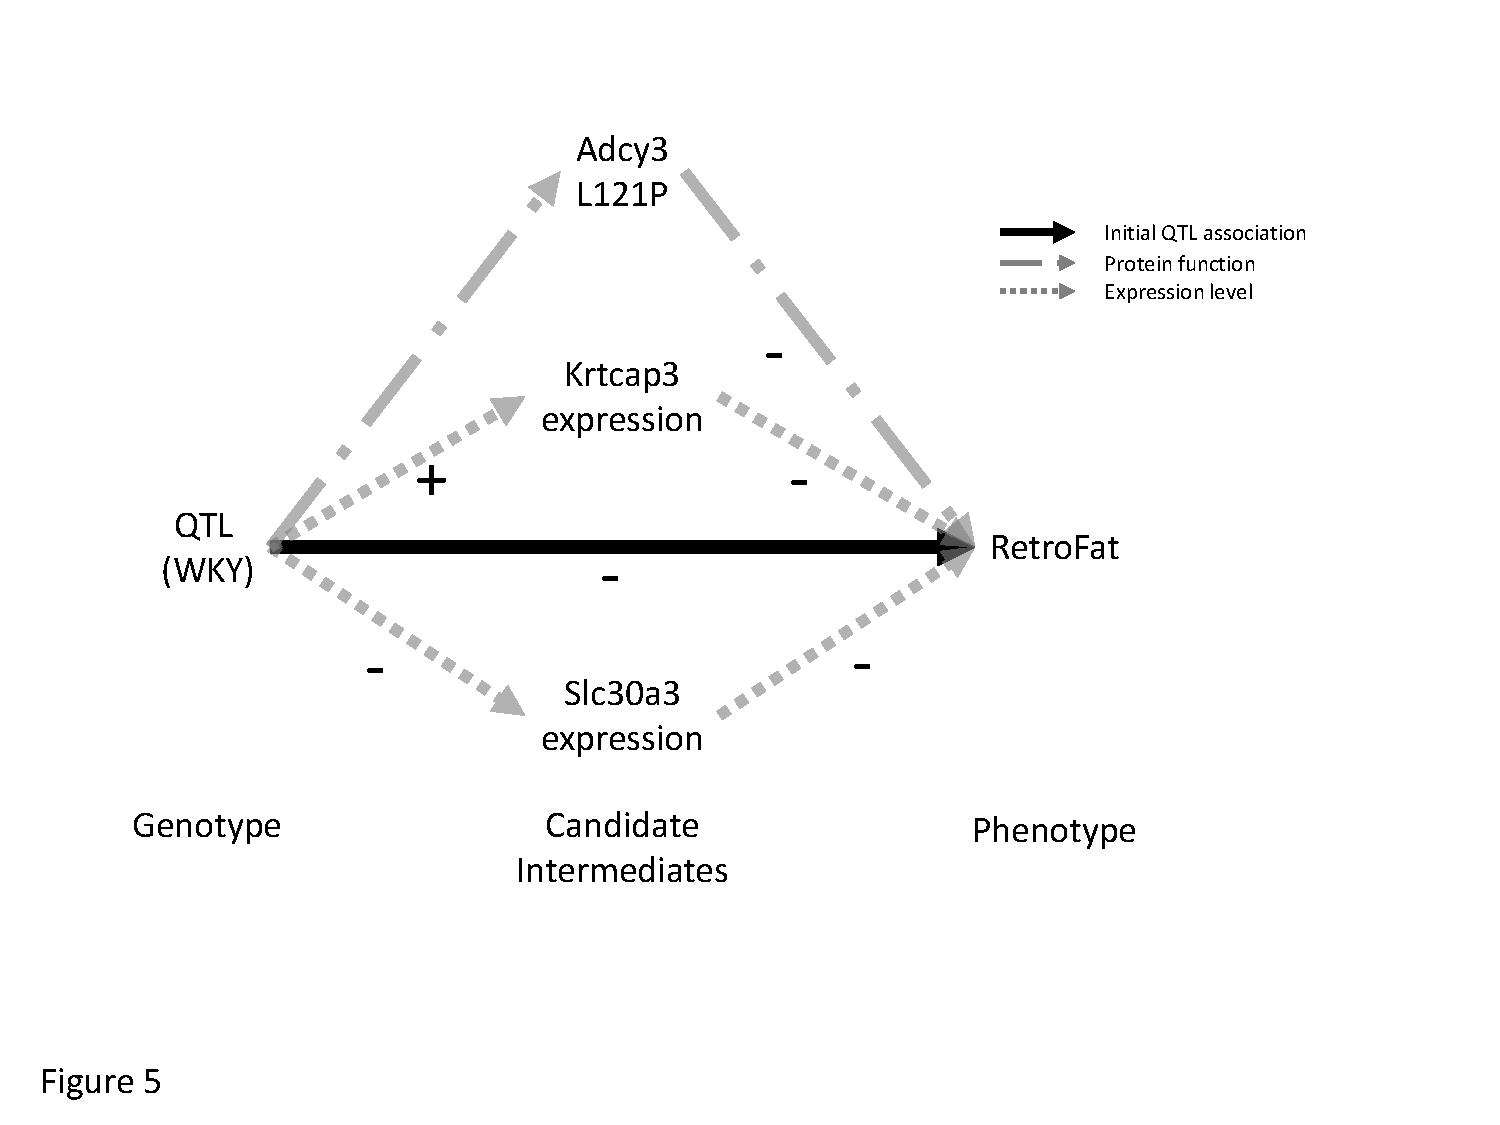
\includegraphics[trim={0in 1.5in 0in 0.5in}, clip, width=\textwidth]{figures/5-hsrats/Figure5.pdf}
\caption[Causal graph model for the candidates underlying the RetroFat chromosome 6 QTL]{Model demonstrating role of \textit{Adcy3}, \textit{Krtcap3} and \textit{Slc30a3} on RetroFat. WKY haplotype increases expression of \textit{Krtcap3}, which is itself negatively correlated with RetroFat (\textbf{Figure \ref{fig:krtcap3}}), and thus the causal path is consistent with the negative WKY effect on RetroFat at the locus.  In contrast, WKY decreases expression of \textit{Slc30a3}, which is also negatively correlated RetroFat, suggesting \textit{Slc30a3} is a suppressor of the QTL/\textit{Krtcap3} effect.  Finally, the non-synonymous variant with \textit{Adcy3} causes amino acid change L121P leading to lower RetroFat. \label{fig:mediation_graph}}
\end{figure}

\subsection{Identification of \textit{Prlhr} within the chromosome 1 RetroFat QTL}

Within the chromosome 1 RetroFat QTL, there are 15 genes, ten of which are uncharacterized (\textbf{Figure \ref{fig:retrofat_chr1}BC}, \textbf{Table \ref{tab:retrofat_chr1_genes_1}} - \textbf{\ref{tab:retrofat_chr1_genes_2}}).  One gene, \textit{Prlhr}, contains a non-synonymous variant in the BUF and WKY founder strains, two founder haplotypes associated with an increase fat pad weight at this locus. The variant falls within the start codon, changing methionine to isoleucine.  The next methionine falls at amino acid 65, such that the conserved N-terminal region and half of transmembrane helix 1 would be deleted with the variant (\textbf{Figure \ref{fig:retrofat_chr1}E}, \url{https://youtu.be/vRTIkITXRbw}). A molecular dynamic simulation of the PRLHR protein with and without the first 64 amino acids showed strong changes to the entire GPCR transmembrane region. \textit{Prlhr} is expressed mainly in adrenal and brain such that expression levels could not be determined in liver tissue.  None of the liver-expressed genes local to the QTL map as cis-eQTL, thus \textit{Prlhr} remains the strongest candidate within this region.

\begin{figure}
\centering
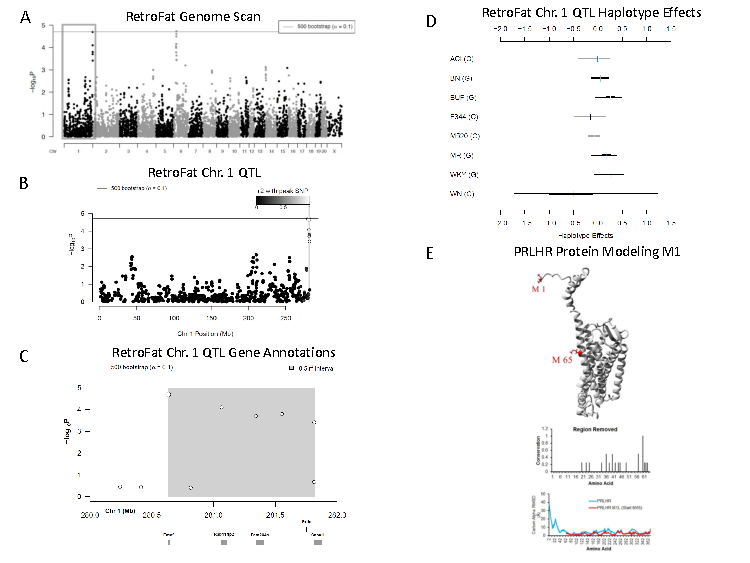
\includegraphics[trim={0in 0in 0in 0in}, clip, width=\textwidth]{figures/5-hsrats/Figure6-alt.pdf}
\caption[RetroFat chromosome 1 QTL and subsequent fine-mapping analyses]{Genome scan of RetroFat as described in \textbf{Figure \ref{fig:retrofat_chr6}A} (A). The grey region highlights the 1.19 Mb LD support interval for the chromosome 1 locus representing neighboring markers that are correlated with the peak marker, representing genomic regions likely to contain the causal variant underlying the statistical signal (B). Annotation of the five characterized genes that fall within the support interval (C). Additive founder haplotype effects for the chromosome 1 RetroFat locus (D). Additive haplotype effects were estimated using the Diploffect model, which takes into account uncertainty in haplotype state. SNP allele information is also overlaid on the haplotype effects. The C allele is shared by ACI, F344, and M520, that possesses a variant with a negative effect on RetroFat, whereas BUF, MR and WKY haplotypes result in increased RetroFat at this locus. Protein modeling for PRLHR (E).  Variant M1I of PRLHR is found within the methionine start site. The next start site is at position 65 leading to removal of the conserved N-terminal region and half of transmembrane helix 1. 16 amino acids removed are under selective pressure (middle panel) and the deletion of the first 64 amino acids causes a destabilization of the entire proteins dynamics as seen by the molecular dynamic simulations (bottom panel). \label{fig:retrofat_chr1}}
\end{figure}

\section{Body weight QTL on chromosome 4 and identification of \textit{Grid2}}

A 95\% significant QTL for body weight was also detected on rat chromosome 4: 91.35Mb to 94.7Mb (3.35 Mb, $\text{logP} = 5.32$) (\textbf{Figure \ref{fig:bodyweight_chr4}ABC}). At this locus, whose effect size was 12.33\%, decreases in body weight were associated with ACI, BUF, F344 and MR haplotypes, and increases with BN (\textbf{Figure \ref{fig:bodyweight_chr4}D}). 

Within the body weight QTL, there are only 11 genes, nine of which are pseudogenes or uncharacterized LOC proteins, leaving only \textit{Ccser1} and \textit{Grid2} (\textbf{Figure \ref{fig:bodyweight_chr4}C}, \textbf{Table \ref{tab:bodyweight_chr4_genes_1}}). None of the genes at this locus contained highly conserved potentially damaging non-synonymous variants. Both \textit{Ccser1} and \textit{LOC108350839} are expressed in liver, but the expression of neither was significantly associated with the body weight QTL, ruling these out as candidate mediators. The brain-specific \textit{Grid2} is the only gene that has previously been linked to body weight \citep{Nikpay2012} and \textit{Grid1} was recently associated with BMI in human GWAS \citep{Locke2015}, implicating \textit{Grid2} as the most likely candidate at this locus. 

\begin{figure}
\centering
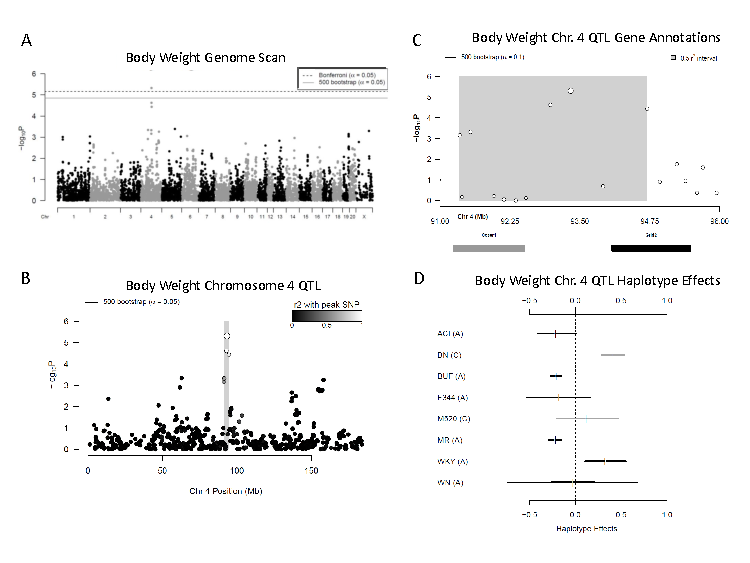
\includegraphics[trim={0in 0in 0in 0in}, clip, width=\textwidth]{figures/5-hsrats/Figure7-alt.pdf}
\caption[Body weight chromosome 4 QTL and subsequent fine-mapping analyses]{Genome scan of body weight (A). X-axis is position on chromosome and y-axis is the logP level of association. Genome-wide significance thresholds were calculated using parametric bootstraps from the null model (significant: $\alpha=0.05$, $\text{logP} = 4.86$) and conservative $\alpha=0.05$ Bonferroni thresholds ($\text{logP} = 5.16$). Linkage disequilibrium support interval in grey is 3.35 Mb (B). Annotation of the two characterized genes that fall within the support interval (C). Additive haplotype effects for chromosome 4 body weight QTL (D).  The C allele at the marker could represent shared haplotype descent between BN and M520, both which have an increasing effect on body weight at this locus. ACI, BUF, F344 and MR haplotypes have a decreasing effect of body weight at this locus, all of which share the A allele.  The WKY and WN also have an A allele and the WKY haplotype has an increasing effect on body weight, while the WN haplotype appears not to effect body weight, although the credible interval of both is fairly large and not well represented in the data at this locus.\label{fig:bodyweight_chr4}}
\end{figure}

\section{Discussion}

This is the first study to map adiposity traits genome-wide using HS rats and demonstrates their utility for uncovering genes and variants likely to impact human adiposity. We identified QTL for RetroFat on rat chromosomes 1 and 6 and a QTL for body weight on chromosome 4.  Using various fine-mapping procedures, we identified three likely candidate genes within the chromosome 6 RetroFat locus: a protein-coding variant within \textit{Adcy3}, and transcriptional regulation of \textit{Krtcap3} and \textit{Slc30a3} that mediate between the QTL and RetroFat. Within the chromosome 1 RetroFat QTL, we identified a variant within \textit{Prlhr} that increases fat pad weight.  Lastly, \textit{Grid2} was identified as the most likely candidate gene within the body weight locus. It is of interest that several of these candidate genes play a role in neural regulation of energy metabolism and/or feeding behavior.

As expected, both the HS founders and the HS population varied for adiposity traits, with BUF showing the highest adiposity and ACI, BN and M520 showing the lowest. As seen in humans \citep{Stunkard1986, Katzmarzyk2000}, these traits were highly heritable.  Also similar to humans \citep{Emdin2017a}, increased body weight, particularly visceral fat pad weight (RetroFat and EpiFat), was significantly associated with several measures of metabolic health in the HS rats, indicating that genes underlying QTL for adiposity traits are likely to contribute to overall metabolic health in HS rats.

Despite high heritability for adiposity traits in this model, we found only three QTL for the five traits that were studied.  The remaining heritability could be attributable to loci of small effect and/or complex genetic architecture that lie below the limit of detection in this study, and this accords with the fact that the QTL we identified were each of relatively large effect (12.33\%, 13.33\% and 11.05\% respectively). The identified QTL also had relatively small LD support intervals (3.35 Mb, 1.19 Mb and 6.14 Mb, respectively), significantly decreasing the number of potential candidate genes within each QTL relative to traditional QTL studies using F2 intercross or backcross animals; the map density, however, was too low for high resolution mapping of the genes within the interval. We expect that increasing both the number of animals used as well as the density of genotyping would serve to uncover additional loci.  

The chromosome 6 RetroFat locus encompassed 6.14 Mb, contained 130 genes and was driven by the WKY haplotype. Using a fine-mapping procedure that allowed for the presence of multiple signals, we identified a 1.46 Mb plausible region for the QTL. \textit{Adcy3} was the only gene in this region to contain a highly conserved, non-synonymous variant in the WKY founder strain that is predicted to be damaging: the leucine-to-proline switch at amino acid 121 would likely induce a bend in the helix leading to altered membrane interactions and binding. In addition, we found that multiple genes within the locus map as eQTL. Subsequent mediation analysis supported roles for \textit{Krtcap3} and \textit{Slc30a3}, with \textit{Krtcap3} expression presenting as a full mediator of the QTL and \textit{Slc30a3} expression as a partial/suppressor mediator. Although little is known about \textit{Krtcap3}, \textit{Slc30a3} is a zinc transporter that plays a role in glucose transport and metabolism \citep{Smidt2009}, and \textit{Adcy3} is an enzyme that catalyzes the cAMP second messenger system and is likely involved in energy homeostasis \citep{Wu2016}.  The POMC/RBJ/ADCY3 region has previously been identified in multiple human GWAS for BMI and obesity \citep{Speliotes2010, Nordman2008, Stergiakouli2014, Wen2012}. Interestingly, a non-synonymous amino acid change (Ser107Pro) in the human \textit{Adcy3} gene \citep{Speliotes2010}, which falls within the same transmembrane helix as the rat variant, has been identified as the causal variant in height-adjusted childhood BMI \citep{Stergiakouli2014}, indicating the same likely causal variant between rat and human. \textit{Adcy3} knock-out and haplo-insufficient mice become obese with age, exhibiting increased food intake and decreased locomotion \citep{Tong2016, Wang2011a}.  In addition, gain of function in \textit{Adcy3} protects against diet-induced obesity \citep{Pitman2014}, further supporting a causal role for this gene.  

The chromosome 1 RetroFat locus encompassed 1.19 Mb, contained 15 genes, with BUF, MR, and WKY haplotypes increasing RetroFat. \textit{Prlhr}, containing a non-synonymous variant in both the BUF and WKY strains, stood out as the most likely candidate gene: the variant fell within the methionine start site and leads to removal of the conserved N-terminal region and half of transmembrane helix 1, likely having a large impact on protein function. This variant is found in several other rat strains including FHH, GK, LEW and SD. \textit{Prlhr} is known to play a role in feeding behavior, with ICV administration in the hypothalamus leading to decreased food intake \citep{Lawrence2000}, and \textit{Prlhr} knock-out mice exhibiting increased food intake, body weight and fat pad weight \citep{Gu2004a}.   Interestingly, this specific variant did not alter feeding behavior in outbred Sprague-Dawley rats \citep{Ellacott2005}, indicating that the effect of the variant on fat pad weight may be independent of food intake, although additional studies are needed to confirm this.

The body weight locus encompassed 3.35 Mb and contained 11 genes, none of which contained highly conserved non-synonymous variants predicted to be damaging between the two haplotype effect groups: ACI, BUR, F344, MR versus BN. Only one gene in the region, \textit{Grid2}, has previously been linked to obesity, jointly with tobacco use, in a family-based study \citep{Nikpay2012}, making it the most likely candidate gene.  Interestingly, \textit{Grid1} was associated with BMI in a recent human GWAS \citep{Locke2015}, further supporting a potentially causal role for \textit{Grid2} within the rat body weight locus. \textit{Grid2} encodes the glutamate ionotropic receptor delta type subunit 2 and is known to play a role in synapse formation, particularly within the cerebellum \citep{Hirai2003}.  Synaptic formation and plasticity are increasingly being recognized as playing a role in metabolism and energy balance \citep{Dietrich2013}.  Additional work, including assessing \textit{Grid2} expression levels in brain, is needed to confirm or eliminate \textit{Grid2} as the causal gene at this locus. 

In summary, we have used HS rats to identify QTL for adiposity traits, leading to identification of five candidate genes and two likely causal variants.  Some genes have previously been identified in human GWAS or linkage studies (\textit{Adcy3}, \textit{Grid2}) or implicated in rodent models of obesity (\textit{Adcy3}, \textit{Prlhr}), while two genes are novel (\textit{Krtcap3}, \textit{Slc30a3}).   The \textit{Adcy3} variant falls within the same transmembrane helix as that found in humans indicating direct human relevance of this work.   It is also of interest that \textit{Adcy3}, \textit{Prlhr} and \textit{Grid2} have previously been found to impact feeding behavior and/or neural regulation of metabolism.  This work demonstrates the power of HS rats for genetic fine-mapping and identification of underlying candidate genes and variants that will likely be relevant to human adiposity.  

\section{Detailed Methods}

\subsection{Animals}

\subsubsection{Housing} 
Rats were housed two per cage in micro-isolation cages in a conventional facility using autoclaved bedding (sani-chips from PJ Murphy). They had \textit{ad libitum} access to autoclaved Teklad 5010 diet (Harlan Laboratories) and were provided reverse osmosis water chlorinated to 2-3 ppm.

\subsection{Statistical genetic analysis}

\subsubsection{Modeling genetic effects on adiposity} 

All statistical genetic analyses described used the same general model (or approximations to it) for linking the genetics of a given rat  to its measured phenotypic outcome. This was the linear mixed effect model (LMM)
\begin{equation}
	f(y_{i}) = \text{covariates}_{i} + \text{QTL}_{i}(m) + u_{i} + \text{residual}_{i}, \label{eq:general_model}
\end{equation}
where, in brief: $f(y_{i})$ is the phenotype subject to a normalizing transformation, specifically, as a conservative measure to rein in high influence data points, we used the rank inverse normal transformation; $\text{covariates}_{i}$ is a fixed effects term that includes variables representing time food deprived, order of tissue harvest, and dissector (notably, dissector significantly affected EpiFat and BMI\_Tail\_Base); $\text{QTL}_{i}(m)$ represents the effect of the quantitative trait locus (QTL) at genomic locus $m$, and is defined in more detail below; and $\text{residual}_{i}$ models the remaining individual-to-individual variation as a normal deviate with variance $\sigma^{2}$. The $u_{i}$ term is a random polygenic effect representing the effect of overall genetic relatedness, modeled as vector $\mathbf{u} = (u_{i}, \ldots, u_{n})$ drawn from a multivariate normal with covariance matrix $\bG\tausq$, where $\tausq$ is unknown and $\bG$ is the realized genetic relationship matrix, estimated as the pairwise distance in allelic dosages defined by the identity by descent (IBD) probabilities from founder haplotypes, standardized by allele frequency and averaged over loci across the genome, calculated using the \texttt{kinship.probs} function in the DOQTL R package \citep{Gatti2014}. The LMM in Eq \ref{eq:general_model} with $\text{QTL}_{i}(m)$ omitted is hereafter referred to as ``the null model".

\subsubsection{Heritability estimation}

Narrow-sense heritability,
\[	
h^{2} = \frac{\tau^{2}}{\tau^{2} + \sigma^{2}} \times 100\%\;,
\]
was estimated for each phenotype by fitting the null model as a Bayesian LMM using INLA \citep{Rue2009a,Holand2013a}, which gives a complete posterior distribution of $h^{2}$, along with point and interval estimates. Phenotypes were scaled to have a mean of 0 and standard deviation of 1, and a uniform prior on $h^{2}$ was obtained by setting priors on $\tau^{-2}$ and $\sigma^{-2}$ to $\text{Ga}(1, 1)$, with other settings being default.

\subsubsection{QTL mapping}

QTL were identified by genome-wide association of imputed SNPs. This was performed in three steps. First, as in previous work \citep{SolbergWoods2012}, we obtained a probabilistic reconstruction of each rat's haplotype mosaic, that is, the configuration of inherited founder haplotypes that compose its genome, using a hidden Markov model (HMM), implemented in R/qtl2geno \citep{Broman2016}, applied to the genotype data on HS rats and their founders. This HMM was used to calculate for each individual $i = 1, \ldots, n$, at each marker position $m = 1, \ldots, 8218$, a vector of 36 descent probabilities, $\mathbf{p}_{im}$, containing the posterior probability of descent from each of the possible $\frac{8(8+1)}{2} = 36$ haplotype pairs (diplotypes). $n$, the sample size, varies between phenotypes, with $n = 989$ for those irrespective of tissue harvest age, such as body weight, and $n = 743$ for those that include only individuals with tissue harvested at 17 weeks of age, such as RetroFat (two rats did not have RetroFat measurements, resulting in $n = 741$). Second, these descent probabilities were used to re-estimate the original SNP genotypes, that is, each $\mathbf{p}_{ij}$ was used to infer a 3-vector of imputed genotype probabilities $\mathbf{g}_{ij}$; these imputed genotypes, which, unlike their raw counterparts, were both complete and relatively robust to genotyping error, were carried forward into subsequent analyses. Third, at each SNP, we fitted the LMM in Eq \ref{eq:general_model}, setting $\text{QTL}_{i}(m) = \beta x_{mi}$ where $x_{mi}$ is the expectation of the minor allele count (ie, the allele dosage) implied by $\mathbf{g}_{im}$, and $\beta$ is a fixed effect; comparing the maximum likelihood (ML) fit of this model to that of the null model gave a likelihood ratio test and nominal p-value, reported as its negative base 10 logarithm, or logP. (Note that initially we used models testing the association between phenotype and haplotype descent, ie, $\mathbf{p}_{im}$, directly, as in the region-wide mapping of \cite{SolbergWoods2012}, but instead used the less complicated SNP modeling due to a combination of uncertainty in haplotype descent and strong imbalances in the estimated haplotype frequencies.) 

Genome-wide significance thresholds for logP scores were estimated by parametric bootstrap samples from the fitted null \citep{Valdar2009,SolbergWoods2010}, with Bonferroni thresholds, which would be highly conservative due to the serial LD structure, calculated for comparison. 

LD intervals for the detected QTL were defined by including neighboring markers that met a set level of LD, measured with the squared correlation coefficient $r^{2}$; we used $r^{2}=0.5$ to define intervals based on the plots of the SNP associations overlaid with LD information.

\subsubsection{Fine-mapping through Group-LASSO with fractional resample model averaging}

To prioritize SNP variants within the RetroFat chromosome 6 QTL interval, we used the multi-SNP modeling method LLARRMA-dawg \citep{Sabourin2015}, which we applied to the imputed SNP genotypes and a population structure-corrected version of the phenotype, namely the phenotypic residuals of the null model. LLARRMA-dawg uses a combination of variable selection and resampling to identify SNPs that have stable, independent associations with the phenotype. Each SNP receives a resample model inclusion probability (RMIP), an estimate of the probability it would be included in a parsimonious multi-SNP model applied to a resampling of the individuals. SNPs with high RMIPs thus represent stronger candidates, and the existence of multiple SNPs with a high RMIP is consistent with the presence of multiple independent signals.

\subsubsection{Estimating haplotype substitution effects at detected QTL}

For detected QTL, the effect of substituting alternate haplotypes and diplotypes was estimated using the Diploffect model \citep{Zhang2014}, which can help identify interesting alleles of the candidate variants near the mapping signal.  Although stability and power, along with the computational demands of a genome-wide analysis, led us to use SNP association for genetic mapping, these were no longer constraints for haplotype effect estimation at an identified QTL. Diploffect is a Bayesian hierarchical approach designed to work with probabilistically inferred haplotype descent, providing shrinkage that mitigates instability from low haplotype frequencies. In addition to the population structure effect in Eq \ref{eq:general_model}, it models two genetic components at the QTL: additive (haplotype) effects, ie the effect of each dose of haplotype (eg WKY); and dominance deviations, those from the additive model for specific combinations of haplotype, (eg, WKY-ACI). Dominance deviations are typically less informed, but their inclusion stabilizes additive effect estimation. Both have their own variance parameters, $\tau^{2}_{\text{add}}$ and $\tau^{2}_{\text{dom}}$, with QTL effect size recorded as the intraclass correlation coefficient 
\[
\rho_{\text{QTL}} = \frac{\tau^{2}_{\text{QTL}}}{\tau^{2}_{\text{QTL}} + \tau^{2} + \sigma^{2}}\;,
\]
where $\tau^{2}_{\text{QTL}} = \tau^{2}_{\text{add}} + \tau^{2}_{\text{dom}}$. The model was fitted using 200 importance samples from INLA \citep{Rue2009a,Holand2013a}, with phenotype transformations and variance component priors set as for heritability estimation above.

\subsubsection{Analysis of RNA-Seq data}

Total RNA was extracted from the livers of 398 of the HS rats using Trizol, followed by library preparation using Illumina TruSeq Stranded mRNA library kit and sequencing on an Illumina HiSeq2500 (Illumina, Inc., San Diego, CA). BN reference genome sequence (genome build Rn6) and GTF files were obtained from Ensembl. RSEM (v1.3.0) \texttt{rsem-prepare-reference} function was used to extract the transcript sequences from the genome \citep{Li2011a} and to build Bowtie2 indices (Bowtie2 v2.2.8) \citep{Langmead2012}.  RSEM \texttt{rsem-calculate-expression} function was then used to execute Bowtie2 to align reads of each sample to the transcriptome prepared above and to compute transcript level and gene level expression abundance.  Trim Galore (\url{http://www.bioinformatics.babraham.ac.uk/projects/trim\_galore/}) was used to perform quality-based trimming with a cutoff at Q=20.  Seven animals were removed due to low number of input reads.

\subsection{Mediation analysis of phenotype, expression, and QTL}

Mediation analysis was used to identify genes with expression levels that mediate the relationship between QTL and physiological phenotype. Expression levels of genes contained within the LD-based QTL intervals were assessed as potential candidates as full mediators (intermediates that completely explain the association between SNP and phenotype) and partial mediators (intermediates that explain some of the association between SNP and phenotype). Similar to \cite{Baron1986} and adapted for genetic data as in \cite{Battle2014}, evidence of mediation was assessed by a series of association tests, presented as a series of steps below, evaluating the relationships between previously mapped phenotype QTL ($X$), some transformation of the expression of level of a candidate mediator gene $j=1,\dots,J$ ($M$), and some transformation of the phenotype ($Y$).
\begin{enumerate}
	% item 1
	\item \textbf{Potential mediators:} The relationship, represented as an arrow, with directionality encoding causality, $X \rightarrow M$ is evaluated for all $J$ candidate genes in the physiological QTL interval with non-zero expression in greater than 0.25 of the $n$ rats by testing for the association between QTL and expression of gene $j$ via the regression model
	\begin{equation}
    	f(\text{gene.expression}_{ij}) = \text{mapped.QTL}_{i} + u_{i} + \text{residual}_{i},
        \label{eq:x_to_m}
    \end{equation}
	where briefly $f(\text{gene.expression}_{ij})$ is the expression level for gene $j$ of rat $i$ subject to some normalizing transformation, often a rank inverse normal transformation, $\text{mapped.QTL}_{i}$ is the effect of the mapped QTL for rat $i$, and $u_{i}$ and $\text{residual}_{i}$ are respectively the polygenic and individual error terms as described in Eq \ref{eq:general_model}. The maximum likelihood fit of the model in Eq \ref{eq:x_to_m} is compared with the null model (same as Eq \ref{eq:x_to_m} with $\text{mapped.QTL}_{i}$ omitted) to produce a likelihood ratio statistic and corresponding p-value. The p-values are converted to q-values using the Benjamini-Hocheberg false discovery rate (FDR) method \citep{Benjamini1995}. $X \rightarrow M$ for gene $j$ is considered satisfied if $\text{q-value}_{j} < 0.1$. A lenient FDR controlling approach to multiple testing is used because the candidate set of genes is constrained to those local to the QTL interval, as well as the mediation analysis including further tests to satisfy mediator status. The set $K$ ($K \leq J$) genes represent candidate mediators, and are also likely co-localizing eQTL to the QTL. 
   % item 2
   \item \textbf{Full mediators:} The relationship $X \indep Y | M$ is representative of $M$ being a full mediator of $X$ on $Y$, suggesting that $X \rightarrow M \rightarrow Y$, specifically that $X$ does not affect $Y$ outside of through $M$. The support for this relationship in the data is evaluated by comparing the following regression models:
   \begin{equation}
   	f(y_{i}) = \text{mapped.QTL}_{i} + f(\text{gene.expression}_{ij}) + u_i + \text{residual}_{i},
    \label{eq:m_to_y_alt}
   \end{equation}
   and
      \begin{equation}
   	f(y_{i}) = f(\text{gene.expression}_{ij}) + u_i + \text{residual}_{i},
    \label{eq:m_to_y_null}
   \end{equation}
    where Eq \ref{eq:m_to_y_alt} is the alternative model and Eq \ref{eq:m_to_y_null} is the null model for a likelihood ratio test. The expression level of gene $k$ is called a full mediator if $\text{p-value}_{k} > 0.05$, representing the situation in which the effect of QTL on the phenotype is fully explained by expression of gene $k$. After testing for all $K$ candidate mediators, $S$ ($0 \leq S \leq K$) full mediators are called.
    % item 3
    \item \textbf{Partial mediators:} The relationship $M \rightarrow Y | X$ is representative of $M$ being a partial mediator of $X$ onto $Y$. To test the support for this relationship, Eq \ref{eq:m_to_y_alt} for each candidate partial mediator $t$ ($T = K - S$) is compared to
    \begin{equation}
    	f(y_{i}) = \text{mapped.QTL}_{i} + u_i + \text{residual}_{i},
        \label{eq:five}
    \end{equation}
	producing a likelihood ratio statistic and p-value. The FDR controlling approach is used again to obtain corresponding q-values. If $\text{q-value}_{t} < 0.1$, expression of gene $t$ is called a partial mediator of the relationship between the QTL and the phenotype. Gene $t$ could also represent an independent effect on the phenotype from the QTL.
    % item 4
    \item \textbf{Consistency of effects:} The consistency of the signs of the effect of the relationships of $X$ through the mediator $M$ onto $Y$ ($X \rightarrow M \rightarrow Y$) with $X$ on $Y$ ($X \rightarrow Y$) was checked for all called mediators. $X \stackrel{+}\rightarrow Y$ means that $X$ causally increases $Y$, whereas $X \stackrel{-}\rightarrow Y$ means that $X$ causally decreases $Y$. Consistent signs for $X \stackrel{+}\rightarrow Y$ would be $X \stackrel{+}\rightarrow M \stackrel{+}\rightarrow Y$ or $X \stackrel{-}\rightarrow M \stackrel{-}\rightarrow Y$. Similarly, for the $X \stackrel{-}\rightarrow Y$ relationship, consistent mediation relationships would be $X \stackrel{+}\rightarrow M \stackrel{-}\rightarrow Y$ or $X \stackrel{-}\rightarrow M \stackrel{+}\rightarrow Y$. Inconsistent signs, also referred to as paradoxical effects, occur when signs of the relationships to and from the mediator are not consistent with the sign of the relationship from $X$ to $Y$, suggesting that $M$ potentially acts as a suppressive mediator of the relationship $X \rightarrow Y$.
\end{enumerate}

The validity of the causal inference from the mediation analysis depends on the underlying relationships following a directed acyclic graph (DAG). If cycles are present in the graph, the causal inference will likely not be valid. Cycles cannot exist with $X \rightarrow Y$ and $X \rightarrow M$ because the QTL genotype is essentially fixed and cannot be modulated by other quantities. Notably the assumption is made that $M \rightarrow Y$, and that $M \leftarrow Y$ does not occur, though it is plausible that a QTL could modulate a phenotype ($X \rightarrow Y$), which leads the phenotype to modulate expression of certain genes ($Y \rightarrow M$). These types of relationships would produce significant associations whose causal directionality would be misinterpreted by the mediation analysis, thus their inference is dependent on the assumption.

\subsection{Mediation analysis results}

Gene expression data from the liver was measured on 398 of the 989 HS rats (all in the cohort with tissue harvested at 17 weeks of life). The three QTL intervals (RetroFat chromosome 1 and chromosome 6 loci and body weight chromosome 4 locus) were evaluated with mediation analysis in an attempt to identify and prioritize possible candidates that could affect the phenotypes through their expression level variation. 

\subsubsection{Body weight chromosome 4 locus}

The QTL interval for this locus contained 11 genes (\textbf{Table \ref{tab:bodyweight_chr4_genes_1}}). Three of these had liver expression measured. The main candidate \textit{Grid2} was not sufficiently expressed (non-zero expression proportion $<$ 0.25) in liver tissue. The expression levels of the other two genes (\textit{Ccser1} and \textit{LOC108350839}) were not significantly associated with the QTL ($X \rightarrow M$ was not satisfied).

\subsubsection{RetroFat chromosome 1 locus}

The QTL interval contained 15 genes (\textbf{Table \ref{tab:retrofat_chr1_genes_1}} and \textbf{\ref{tab:retrofat_chr1_genes_2}}), of which 5 were contained in the expression data (\textit{Emx2}, \textit{Rab11fip2}, \textit{Fam204a}, \textit{Prlhr}, and \textit{Cacul1}). \textit{Emx2} and the primary candidate \textit{Prlhr} were not sufficiently expressed in the liver. Similar to as in body weight, the  expression levels of the remaining three genes were not significantly associated with the QTL.

\subsubsection{RetroFat chromosome 6 locus}

The interval for this QTL is much wider than the previous intervals, and contains 130 genes (\textbf{Table \ref{tab:retrofat_chr6_genes_1}}-\textbf{\ref{tab:retrofat_chr6_genes_4}}), of which 114 were measured in the liver expression data. Of the 114, 36 genes had non-zero expression below 0.25, leaving 78 genes for which to evaluate $X \rightarrow M$. 14 genes (\textbf{Table \ref{tab:retrofat_chr6_potential_mediators}}) had a significant association ($\text{q-value} < 0.1$) between expression levels and the QTL. These 14 candidate mediators were then tested for evidence of being full mediators. \textit{Krtcap3} was called a full mediator (p-value = 0.15). The remaining 13 were evaluated as partial mediators, resulting in 5 genes being selected ($\text{q-value} < 0.1$) (\textbf{Table \ref{tab:retrofat_chr6_candidate_mediators}}). As \textit{Krtcap3} was a strong candidate as a full mediator, we replaced the QTL in the model of RetroFat with it. Each partial mediator was then individually included in a regression model of RetroFat with \textit{Krtcap3} and compared to the null model with only \textit{Krtcap3} (\textbf{Table \ref{tab:retrofat_chr6_candidate_mediators}}). Only \textit{Slc30a3} remained significant, suggesting that it is the best candidate as an additional regulator of RetroFat, potentially separately from the QTL/\textit{Krtcap3} signal.

\section{Additional Figures}

\begin{figure}
\centering
\includegraphics[page=1, width=0.61\textwidth]{figures/5-hsrats/{SuppFig1.pc.plots.multipanel}.pdf}
\includegraphics[trim={0in 1in 0in 0in}, clip, page=2, width=0.61\textwidth]{figures/5-hsrats/{SuppFig1.pc.plots.multipanel}.pdf}
\caption[First ten principal components comparing genotypes between two genotyping centers]{Principal component analysis for the first ten principal components of genotypes between two genotyping centers. Those genotyped at Hudson Alpha are plotted in red and those genotyped at Vanderbilt are plotted in blue. For all plots, red and blue points fall within the same general region indicating that there are no systematic differences in genotype between the two centers. \label{fig:pca}}
\end{figure}

\begin{figure}
\centering
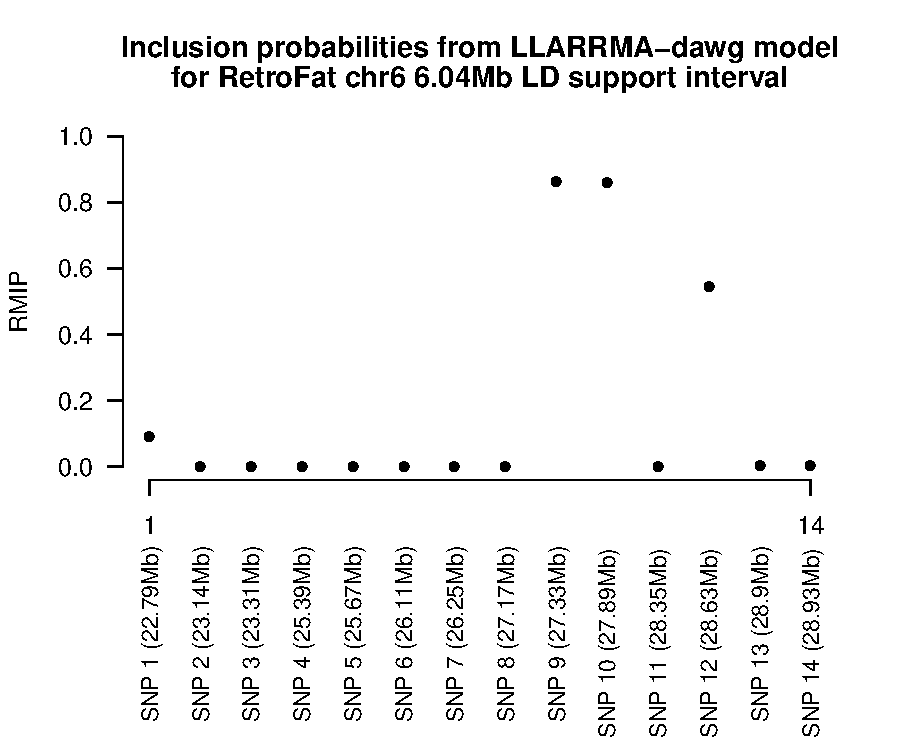
\includegraphics[width=\textwidth, trim={0in 0in 0in 0.75in}, clip]{figures/5-hsrats/RetroFatg_chr6_finemapping_grayscale.pdf}
\caption[Fine-mapping of the RetroFat chromosome 6 QTL with LLARRMA-dawg]{Fine-mapping of the chromosome 6 locus using LLARRMA-dawg reduced the LD support interval from 6.14 Mb to 1.46 Mb. LLARRMA-dawg jointly models and selects SNPs in a region, and returns probabilities corresponding to how often a SNP was included over many re-samples of the data (RMIP). Multiple SNPs with high RMIP suggests the potential for multiple independent signals beneath the QTL peak.\label{fig:llarrma}}
\end{figure}

\begin{figure}
\centering
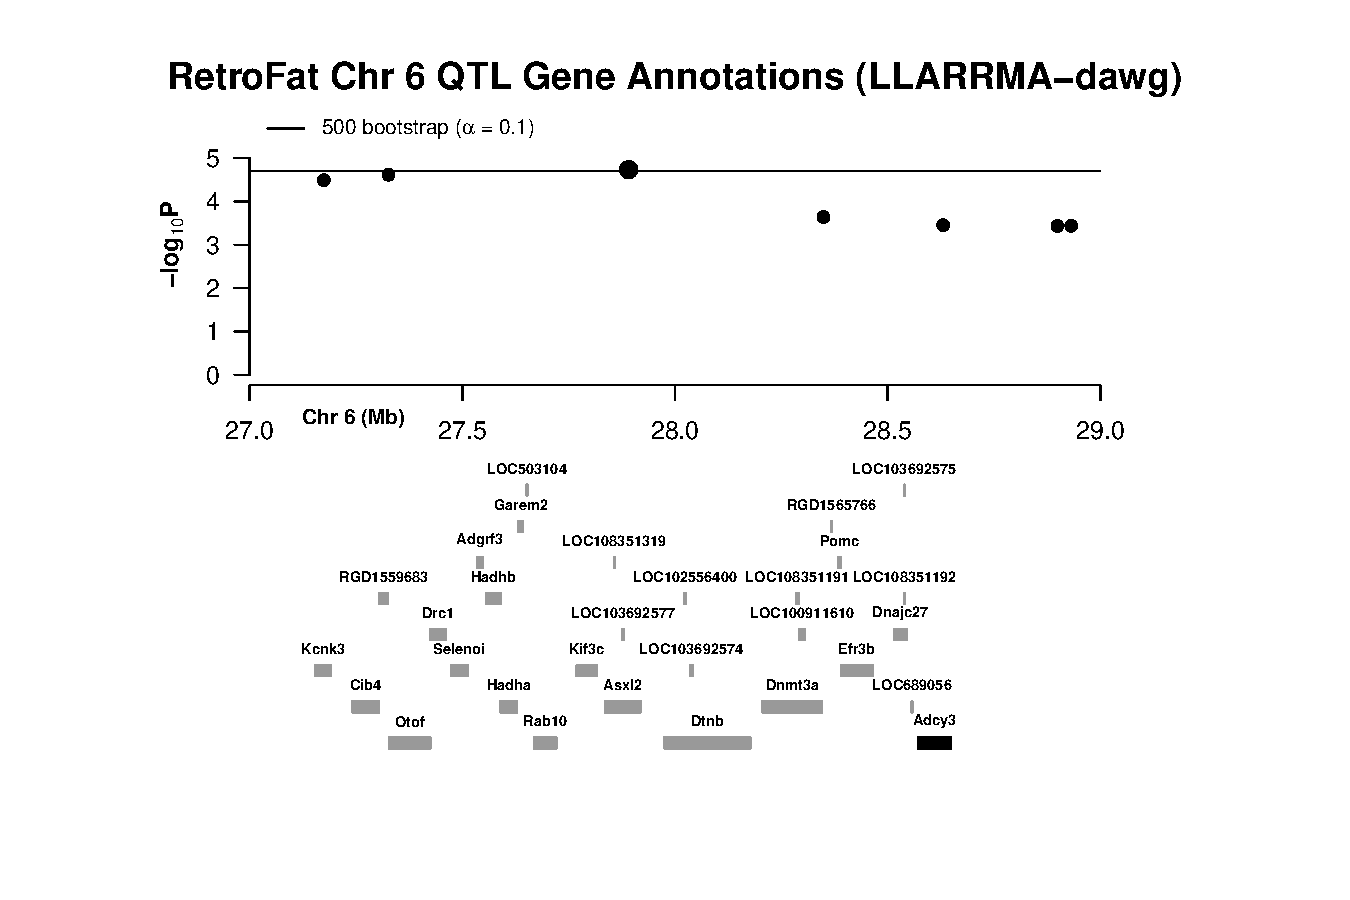
\includegraphics[width=\textwidth, trim={0in 1in 0 0.75in}, clip]{figures/5-hsrats/RetroFat_chr6_finemap_annotations.pdf}
\caption[Gene annotations for the LLARRMA-dawg fine-mapping interval]{The SNP association (7 markers) present in the LLARRMA-dawg fine-mapping interval (\textbf{Figure \ref{fig:llarrma}}), including the annotations of the 30 genes local to the region. The candidate gene \textit{Adcy3} is in bold, and possesses a non-synonymous WKY variant that is predicted to alter protein function (\textbf{Figure \ref{fig:retrofat_chr6}E}).\label{fig:annotations}}
\end{figure}

\begin{figure}
\centering
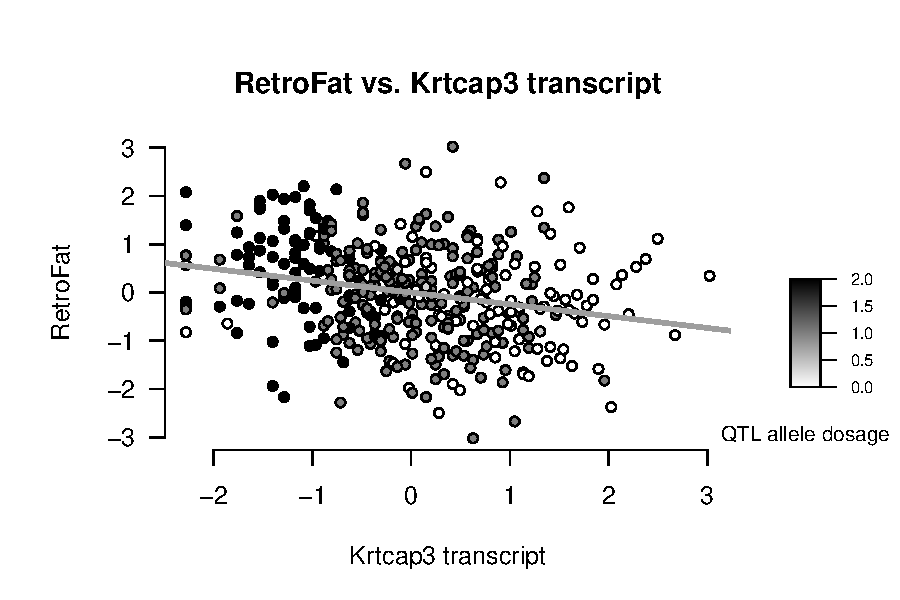
\includegraphics[width=\textwidth, trim={0in 0in 0 0.75in}, clip]{figures/5-hsrats/Krtcap3_scatter.pdf}
\caption[Scatterplot of RetroFat by \textit{Krtcap3} shows signs of direct mediation]{Scatterplot of RetroFat and \textit{Krtcap3} expression levels, with data points colored by the peak SNP minor allele dosages at the QTL. RetroFat and expression levels are rank-inverse normal transformed. \textit{Krtcap3} expression is negatively correlated with RetroFatg (negative trend line). Genotype dosage of the QTL peak SNP is positively associated with RetroFat, and negatively associated with \textit{Krtcap3} expression, which matches \textbf{Figure \ref{fig:mediation_graph}}. \label{fig:krtcap3}}
\end{figure}

\begin{figure}
\centering
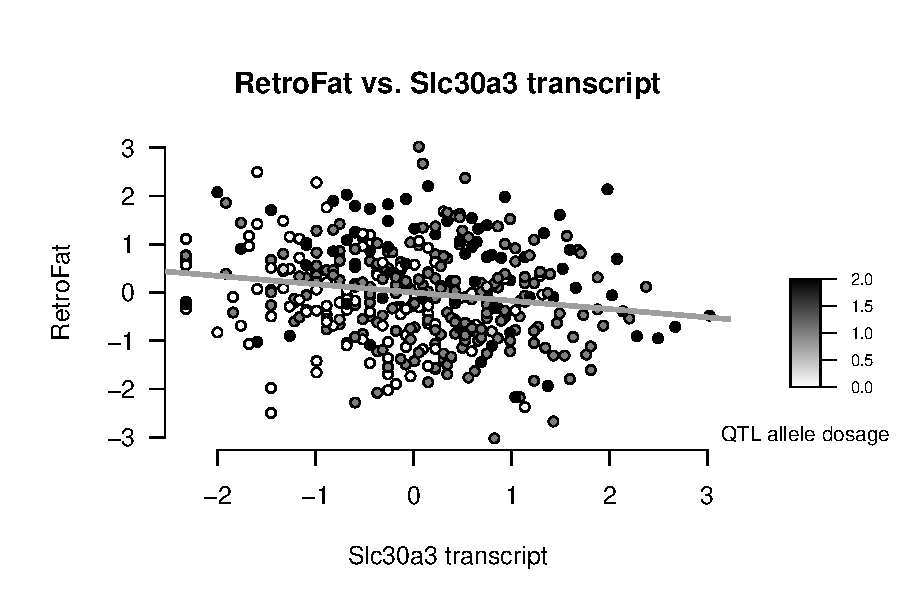
\includegraphics[width=\textwidth, trim={0in 0in 0 0.75in}, clip]{figures/5-hsrats/Slc30a3_scatter.pdf}
\caption[Scatterplot of RetroFat by \textit{Slc30a3} suggests a suppressor]{Scatterplot of RetroFat and \textit{Slc30a3} expression levels, with data points colored by the peak SNP minor allele dosages at the QTL. RetroFat and expression levels are rank-inverse normal transformed.In contrast to \textit{Krtcap3}, the peak SNP minor allele dosage is positive associated with \textit{Slc30a3}, although its expression is negatively correlated with RetroFatg (negative trend line). The mediation path through \textit{Slc30a3} is inconsistent with the QTL relationship with RetroFat, suggesting that \textit{Slc30a3} may actually act in a suppressive manner with respect to the QTL effect. \label{fig:slc30a3}}
\end{figure}

%\subsection{Tables}

\begin{table}
\centering
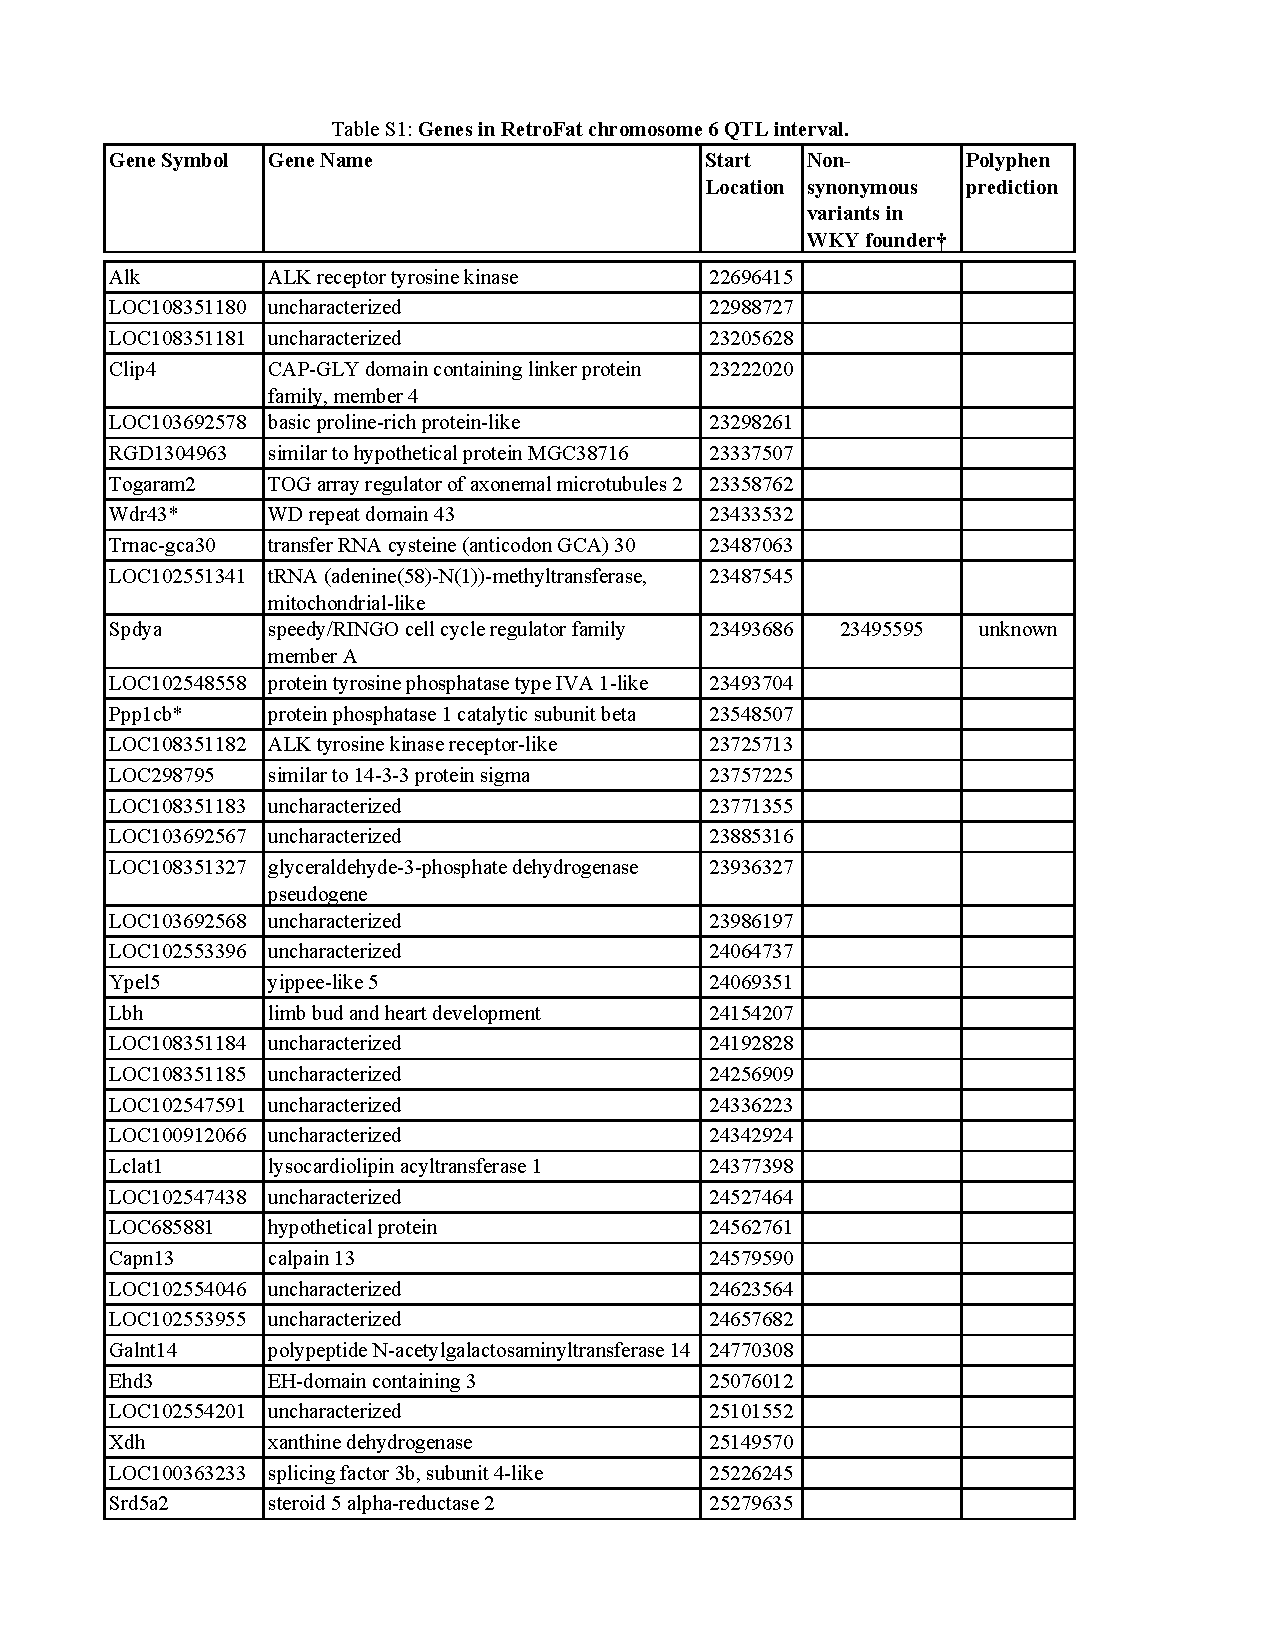
\includegraphics[page=1, trim={0in 0in 0in 0.95in}, clip, width=\textwidth]{figures/5-hsrats/supp_table_retrofat_chr6.pdf}
\caption{Genes in RetroFat chromosome 6 QTL interval \label{tab:retrofat_chr6_genes_1}}
\end{table}

\clearpage

\begin{table}
\centering
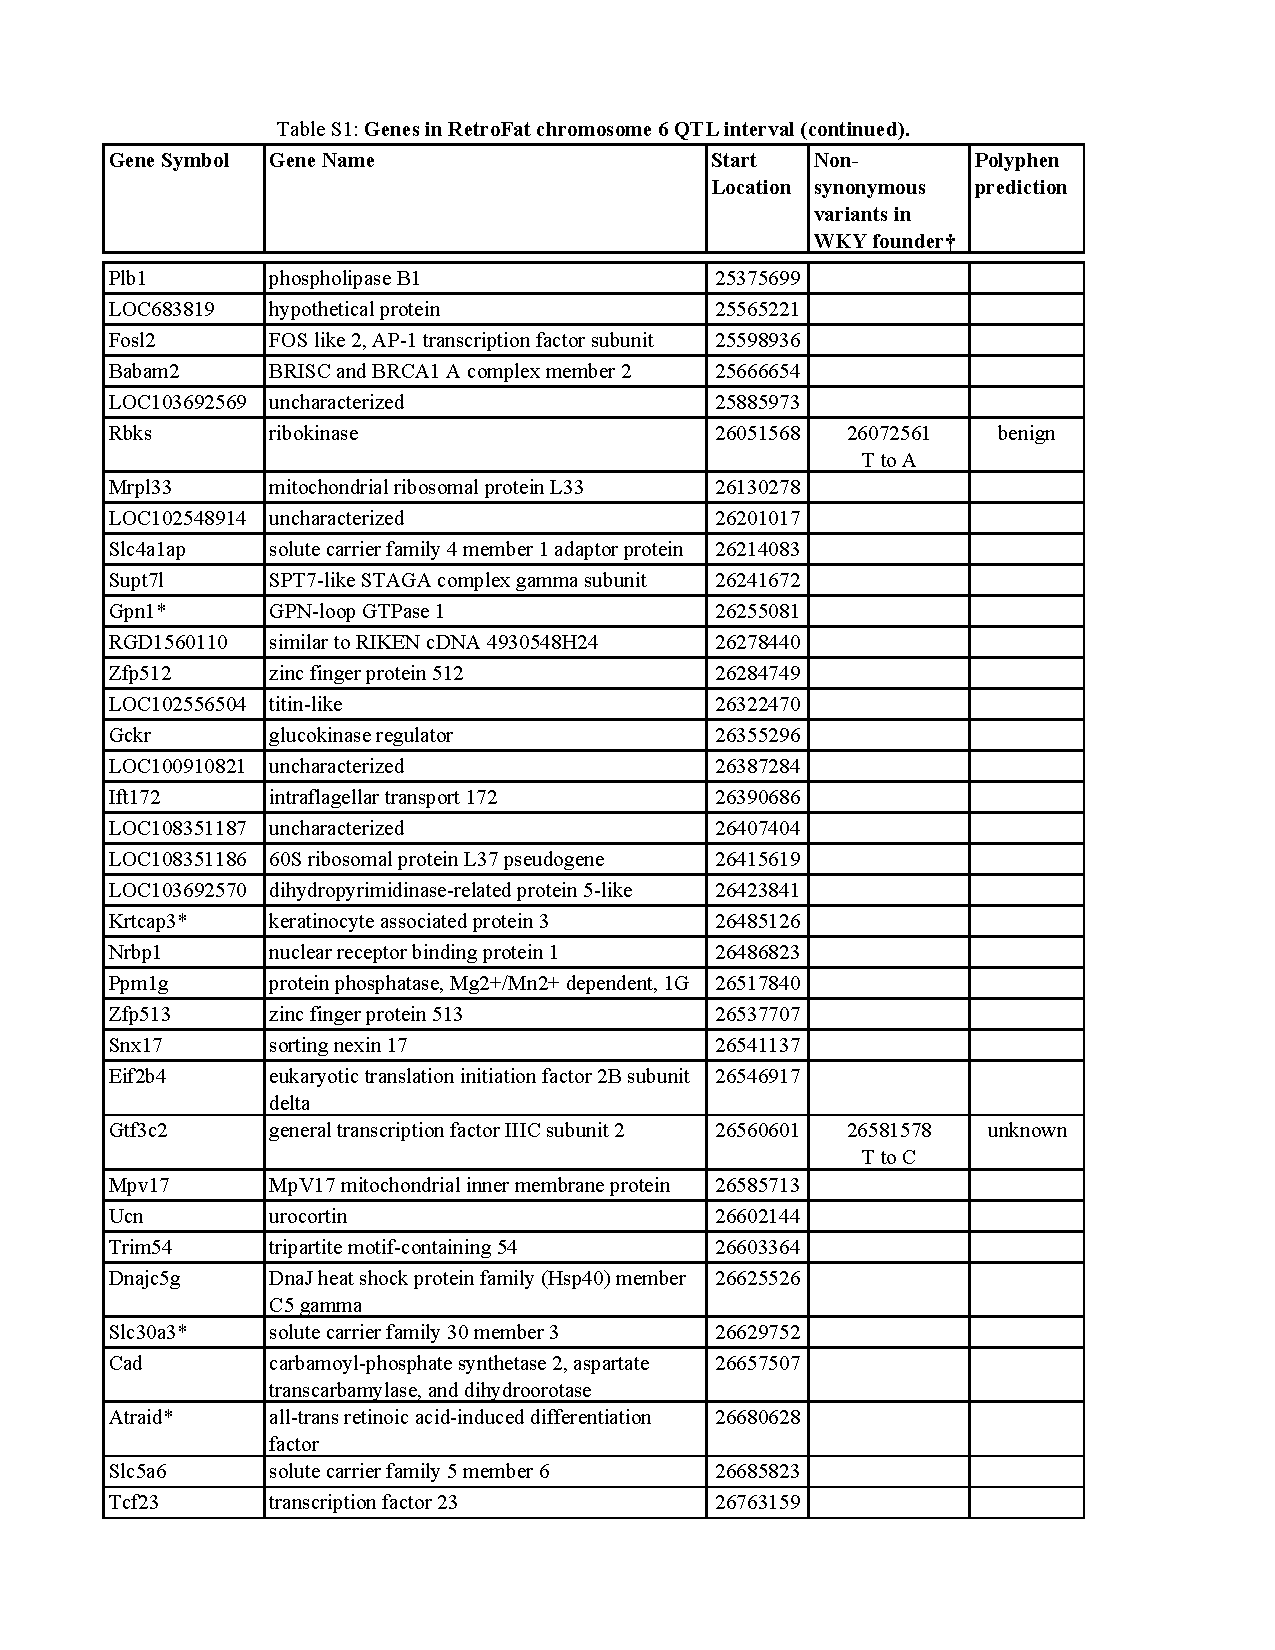
\includegraphics[page=1, trim={0in 0in 0in 0.95in}, clip, width=\textwidth]{figures/5-hsrats/supp_table_retrofat_chr6_extended.pdf}
\caption{Genes in RetroFat chromosome 6 QTL interval (continued) \label{tab:retrofat_chr6_genes_2}}
\end{table}

\clearpage

\begin{table}
\centering
\includegraphics[page=2, trim={0in 0in 0in 0.95in}, clip, width=\textwidth]{figures/5-hsrats/supp_table_retrofat_chr6_extended.pdf}
\caption{Genes in RetroFat chromosome 6 QTL interval (continued) \label{tab:retrofat_chr6_genes_3}}
\end{table}

\clearpage

\begin{table}
\centering
\includegraphics[page=3, trim={0in 2in 0in 0.95in}, clip, width=\textwidth]{figures/5-hsrats/supp_table_retrofat_chr6_extended.pdf}
\caption{Genes in RetroFat chromosome 6 QTL interval (continued) \label{tab:retrofat_chr6_genes_4}}
\end{table}

\clearpage

\begin{table}
\centering
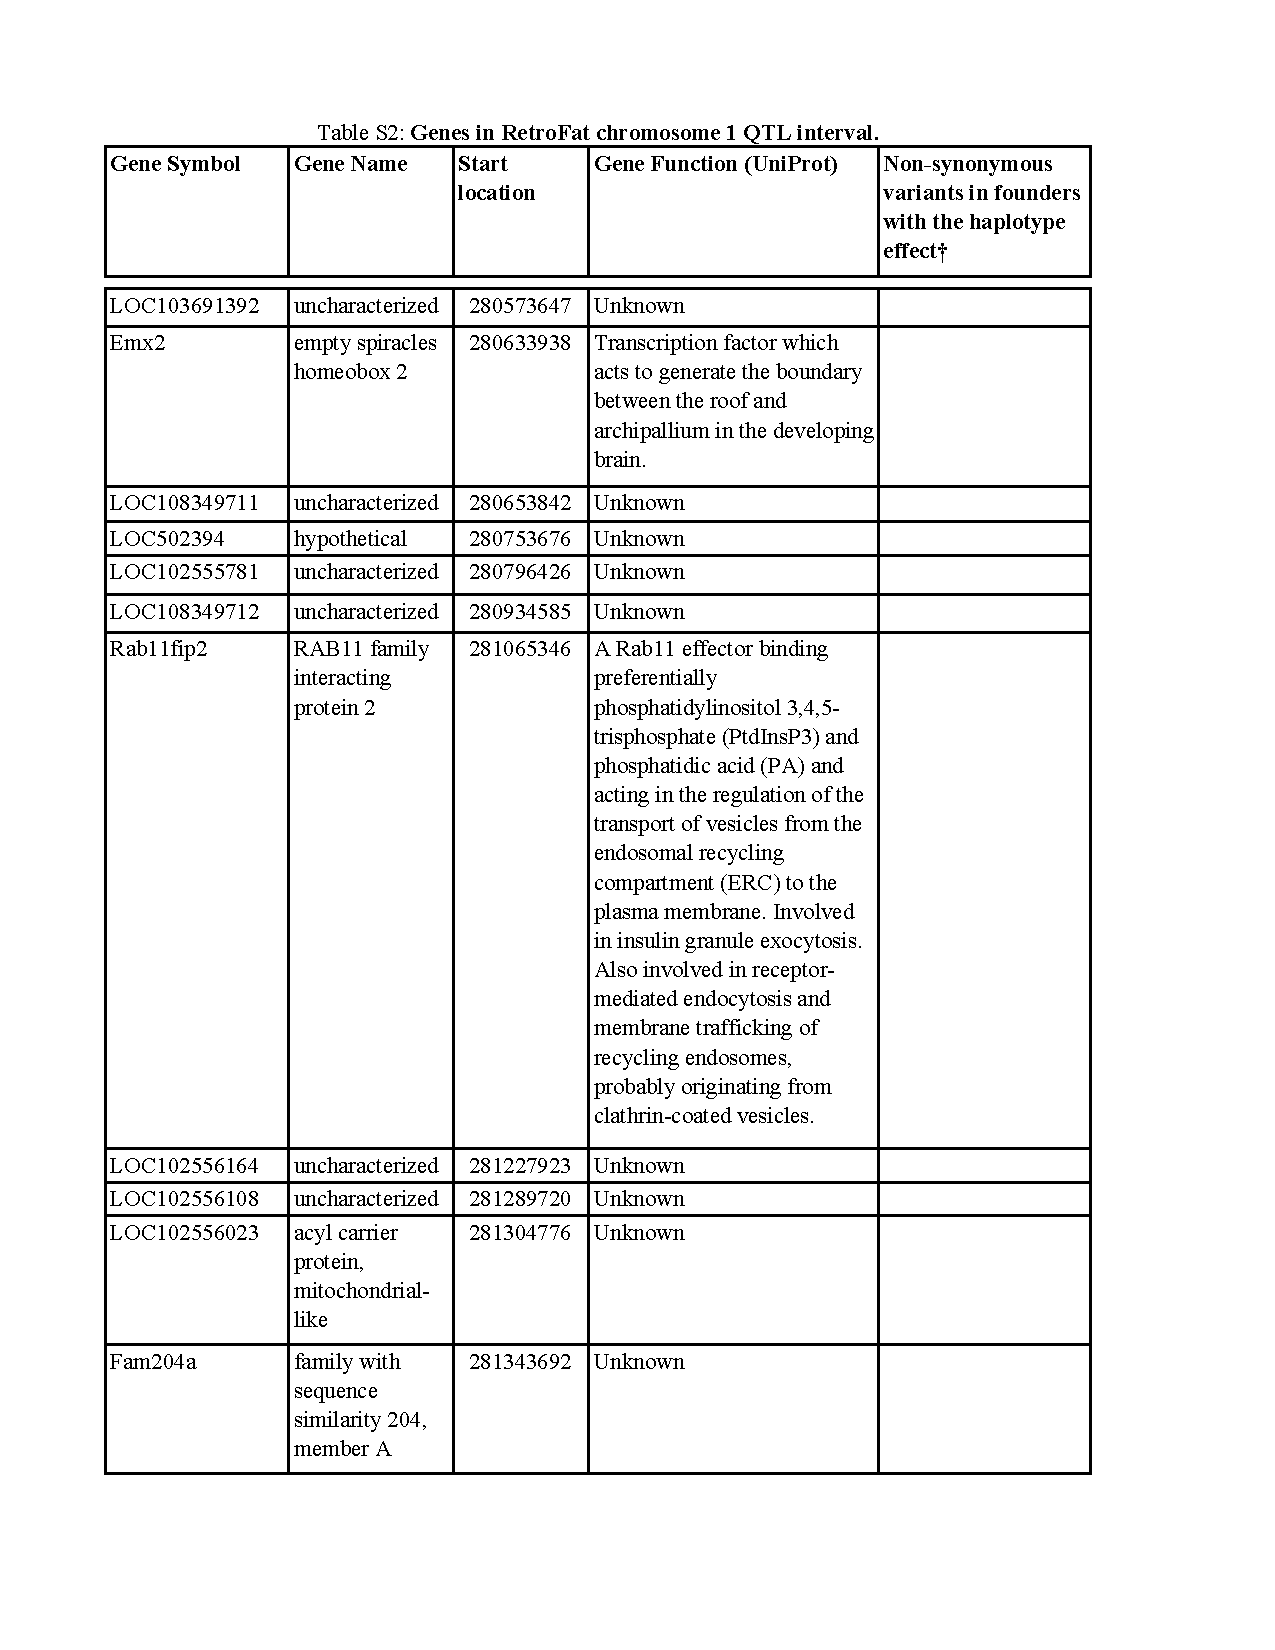
\includegraphics[page=1, trim={0in 0in 0in 0.95in}, clip, width=\textwidth]{figures/5-hsrats/supp_table_retrofat_chr1.pdf}
\caption{Genes in RetroFat chromosome 1 QTL interval \label{tab:retrofat_chr1_genes_1}}
\end{table}

\clearpage

\begin{table}
\centering
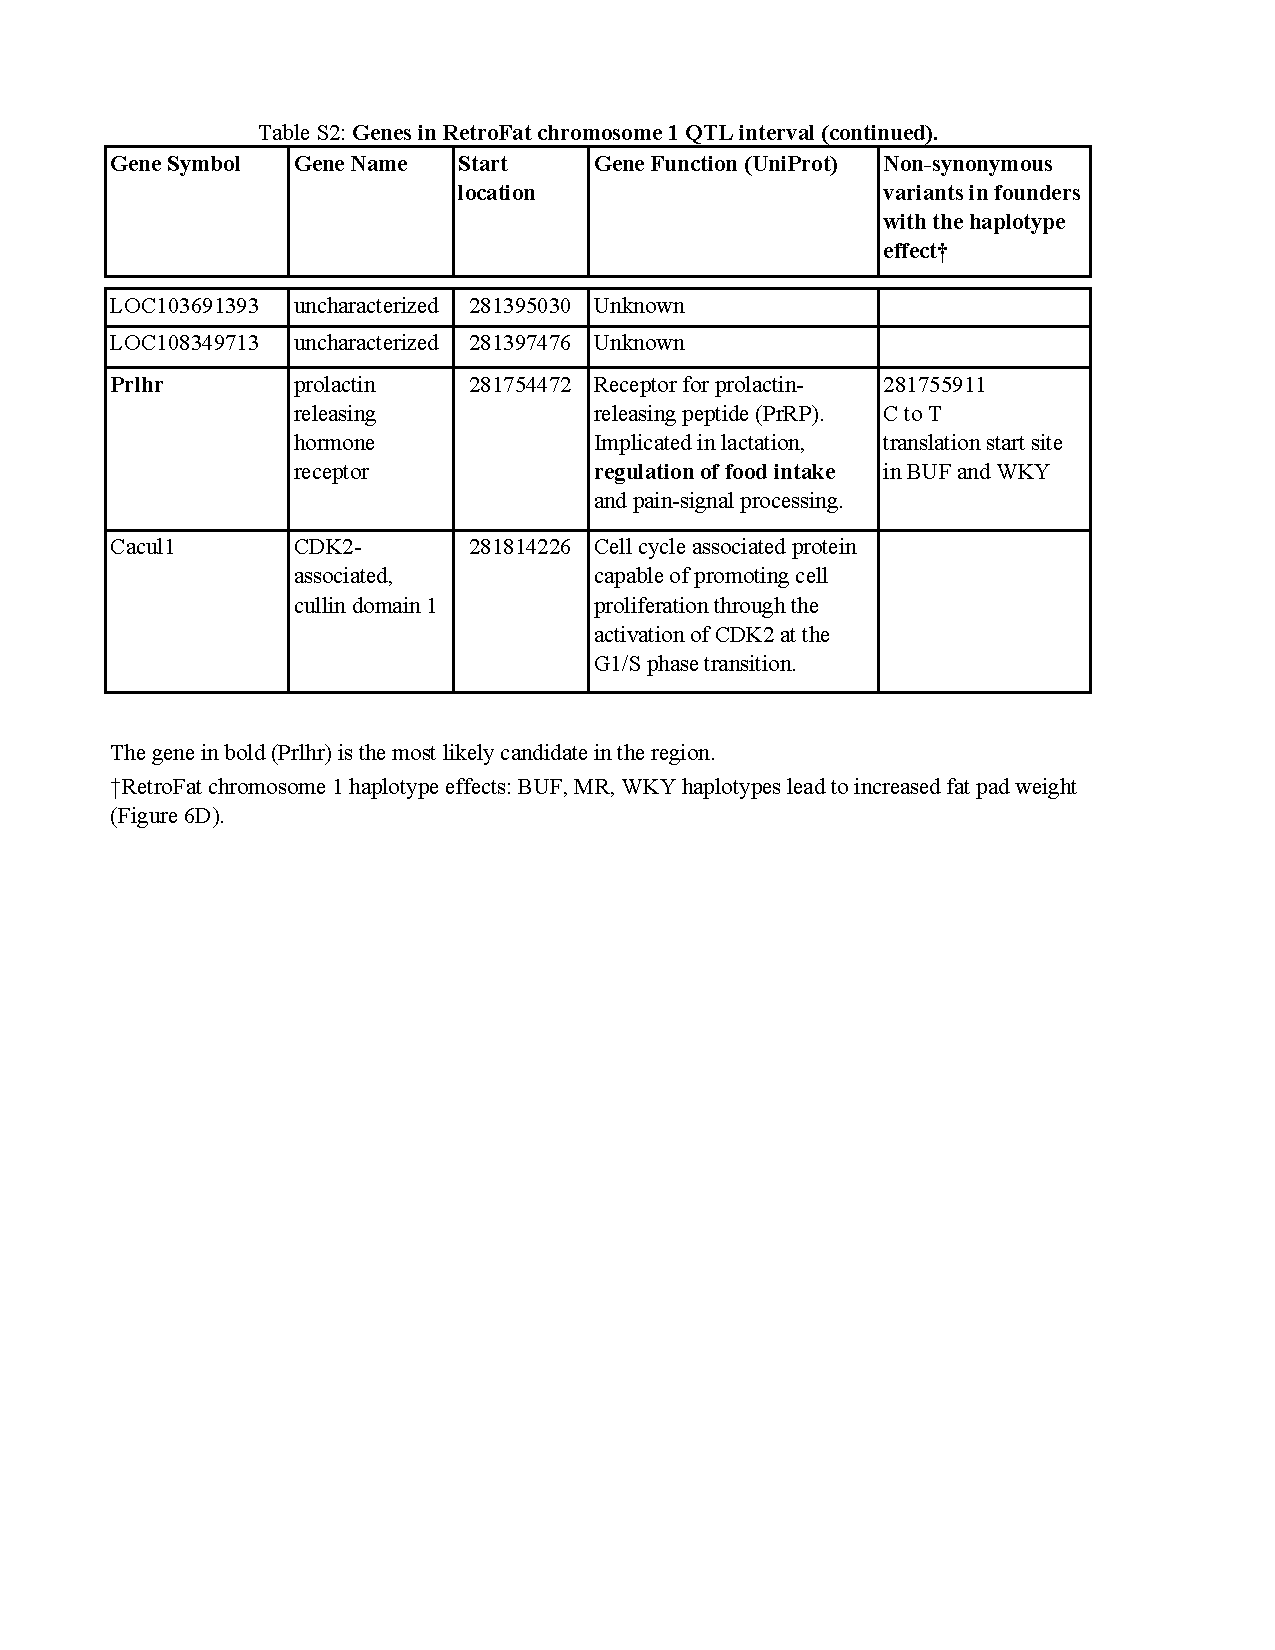
\includegraphics[page=1, trim={0in 5in 0in 0.95in}, clip, width=\textwidth]{figures/5-hsrats/supp_table_retrofat_chr1_extended.pdf}
\caption{Genes in RetroFat chromosome 1 QTL interval (continued) \label{tab:retrofat_chr1_genes_2}}
\end{table}

\clearpage

\begin{table}
\centering
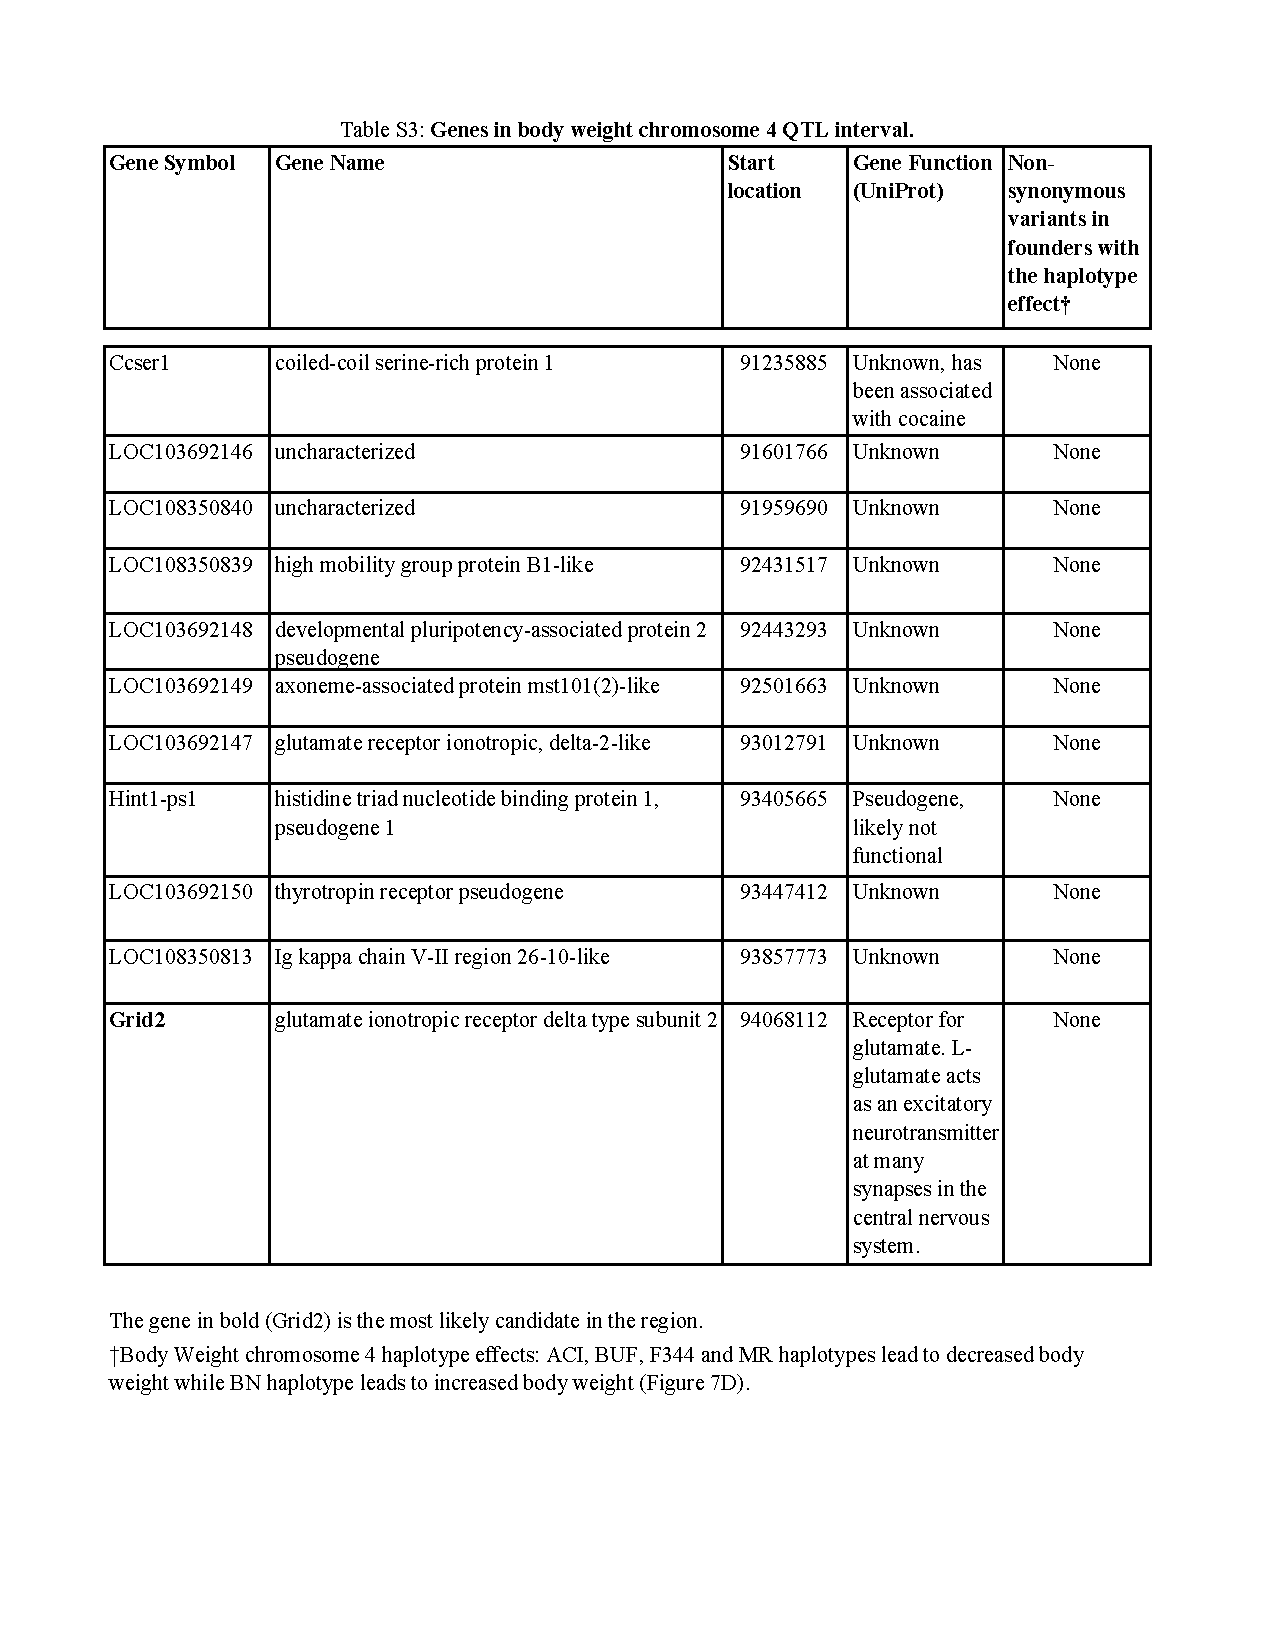
\includegraphics[page=1, trim={0in 1.5in 0in 0.95in}, clip, width=\textwidth]{figures/5-hsrats/supp_table_bodyweight_chr4.pdf}
\caption{Genes in body weight chromosome 4 QTL interval \label{tab:bodyweight_chr4_genes_1}}
\end{table}

\clearpage

\begin{table}
\centering
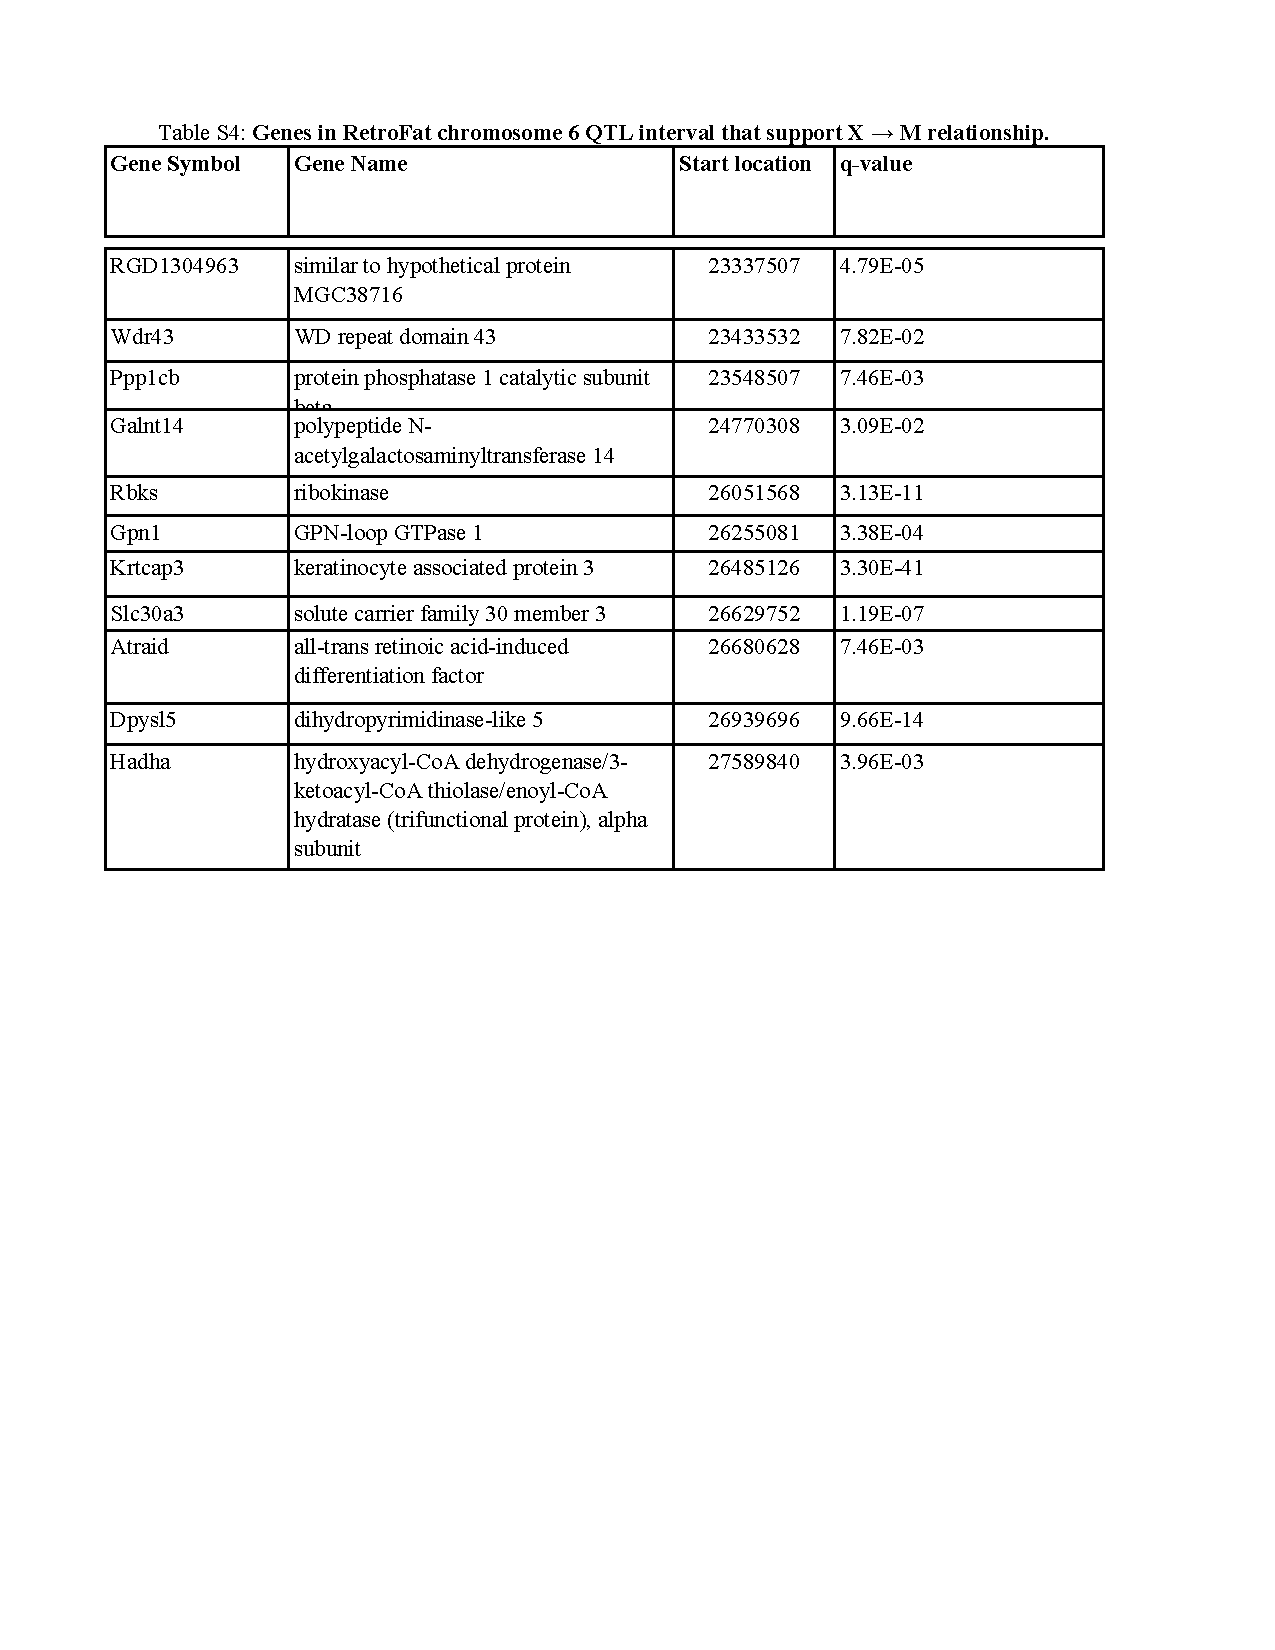
\includegraphics[page=1, trim={0in 5in 0in 0.95in}, clip, width=\textwidth]{figures/5-hsrats/supp_table_eqtl.pdf}
\caption{Potential mediators in RetroFat chromosome 6 QTL interval \label{tab:retrofat_chr6_potential_mediators}}
\end{table}

\clearpage

\begin{table}
\centering
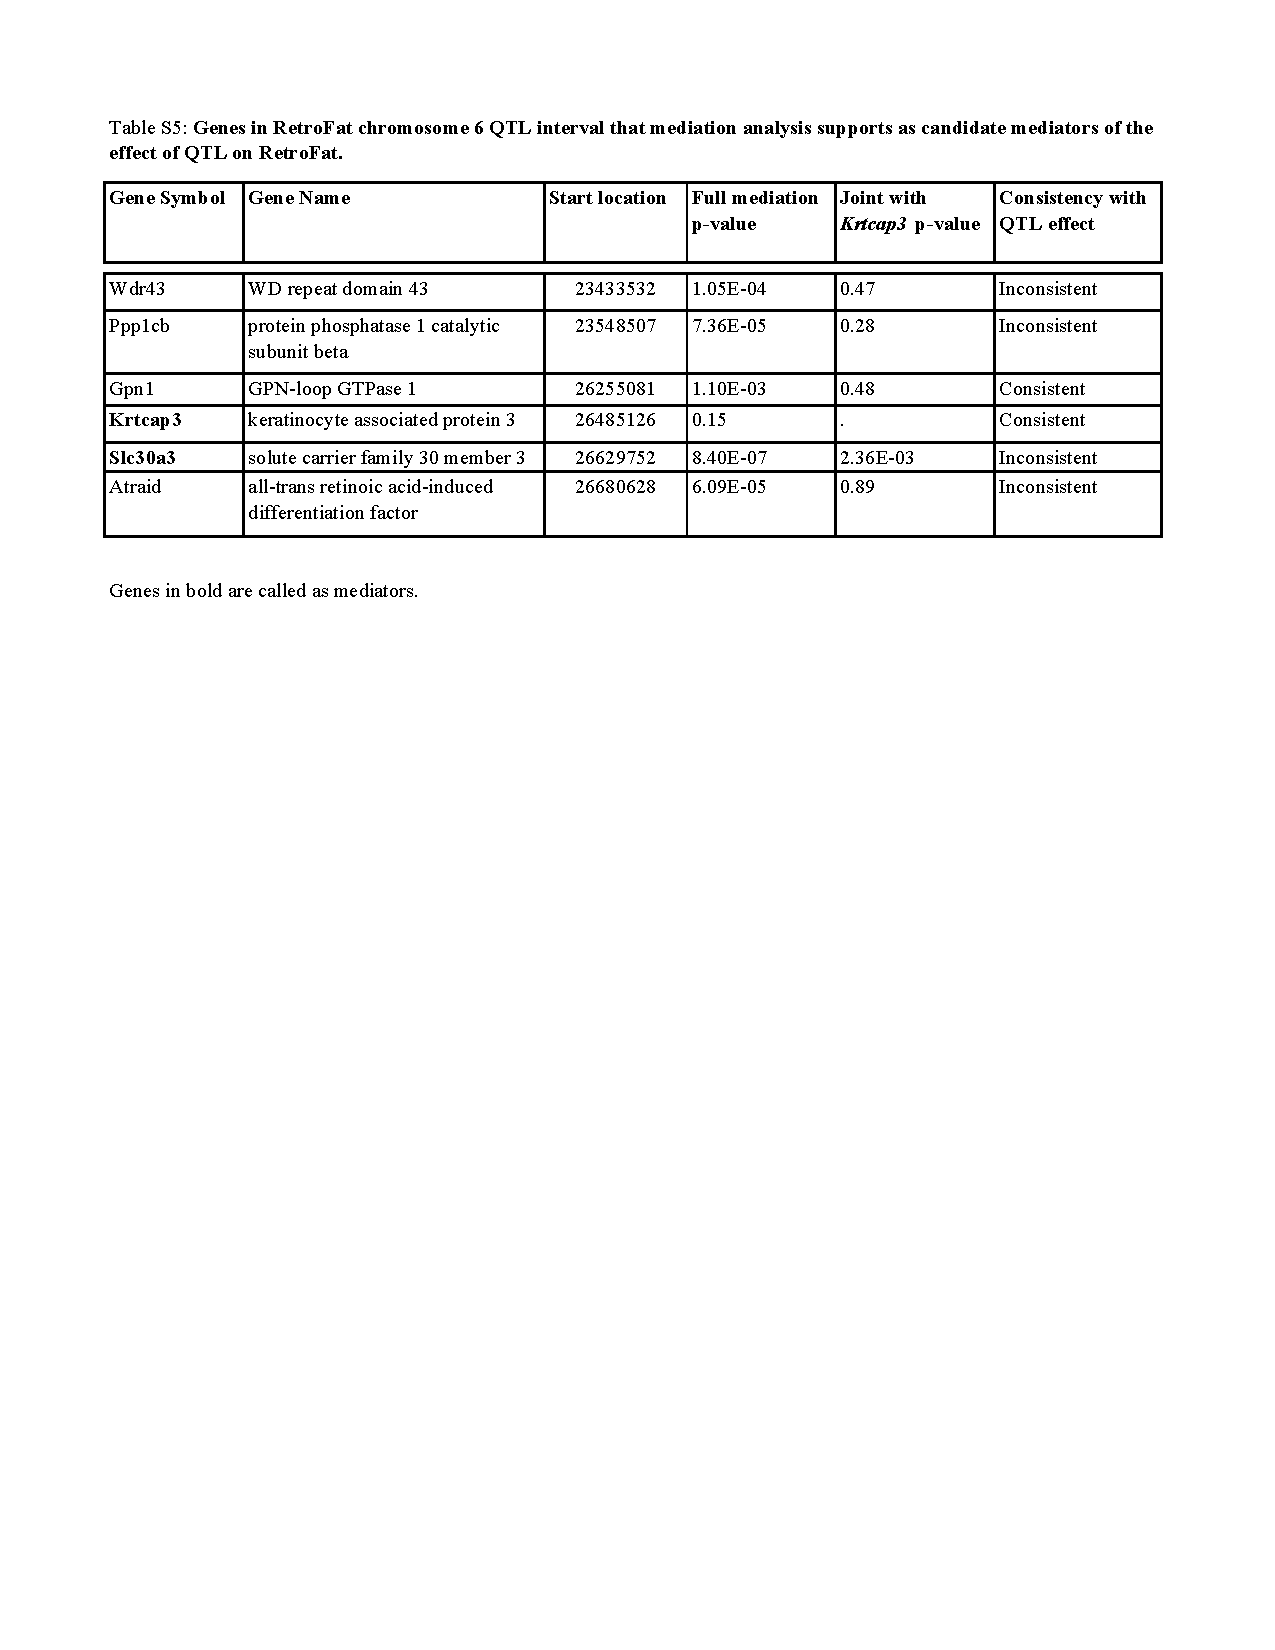
\includegraphics[page=1, trim={0in 7in 0in 1.2in}, clip, width=\textwidth]{figures/5-hsrats/supp_table_mediators.pdf}
\caption{Candidate mediators of the RetroFat chromosome 6 QTL \label{tab:retrofat_chr6_candidate_mediators}}
\end{table}

